%TODO Translate all "Table" and "Figure" of captions .
%TODO Translation of math elements: lim -> lím. sin -> sen. Olso in graphics.

\section{La constante de la circunferencia} % (fold)
\label{sec:the_circle_constant}

\href{http://tauday.com/tau-manifesto}{\emph{El manifiesto tau}} está dedicado a uno de los números más importantes en matemáticas, quizá \emph{el más} importante: la \emph{constante de la circunferencia}, que relaciona su perímetro con su dimensión lineal. Desde hace miles de años, se ha considerado a la circunferencia como la más perfecta de todas las formas, y esta constante condensa su geometría en un único número. Claramente, la opción tradicional para la constante de la circunferencia ha sido $\pi$---pero, como señala el matemático \href{http://www.math.utah.edu/~palais}{Bob Palais} en su delicioso artículo ``$\pi$ Is Wrong!'',\footnote{Palais, Robert. ``$\pi$ Is Wrong!'', \emph{The Mathematical Intelligencer}, volumen~23, número~3, 2001, pp.~7--8. Muchos de los alegatos de \emph{El manifiesto tau} están basados en, o inspirados por, ``$\pi$ Is Wrong!''. Está disponible online en \href{http://www.math.utah.edu/~palais/pi.html}{http://bit.ly/pi-is-wrong}.} $\pi$ \emph{es un error}. Es hora de hacer justicia.

  \subsection{Una propuesta poco modesta} % (fold)
  \label{sec:an_immodest_proposal}

Comencemos a reparar el daño desatado por $\pi$ tratando de comprender en primer lugar el famoso número en sí. La definición tradicional para la constante de la circunferencia establece que $\pi$ (pi) es la razón entre el perímetro de una circunferencia y su diámetro:\footnote{El símbolo $\equiv$ significa ``se define como''.}
\begin{equation}
\label{eq:pi}
\pi \equiv \frac{C}{D} = 3.14159265\ldots
\end{equation}
El número $\pi$ tiene muchas propiedades notables ---entre otras cosas, es un número \href{https://es.wikipedia.org/wiki/Número_irracional}{\emph{irracional}} y de hecho \href{https://es.wikipedia.org/wiki/Número_trascendente}{\emph{trascendente}}--- y aparece por doquier en fórmulas matemáticas.

%TODO Translate image
\begin{figure}
\image{images/figures/circle.pdf}
\caption{Anatomía de una circunferencia.\label{fig:circle}}
\end{figure}

Es obvio que $\pi$ no es ``un error'' en el sentido de ser factualmente incorrecto; el número $\pi$ está perfectamente bien definido, y posee todas las propiedades que las y los matemáticos habitualmente le atribuyen. Cuando decimos que ``$\pi$ es un error'', queremos decir que \emph{$\pi$ es una elección confusa y poco natural para la constante de la circunferencia}. Particularmente, una circunferencia se define como el lugar geométrico de los puntos de un plano que se encuentran a una distancia fija ---el \emph{radio}--- de un punto dado, el \emph{centro} (Figure~\ref{fig:circle}). Así como hay infinitas formas con diámetro constante (figura~\ref{fig:bicycle_constant_diameters}), solo hay una forma con radio constante, lo cual parece sugerir que una definición más natural para la constante de la circunferencia podría utilizar $r$ en lugar de $D$:
\begin{equation}
\label{eq:circle_constant}
\mbox{constante de la circunferencia} \equiv \frac{C}{r}.
\end{equation}
Como el diámetro de una circunferencia es el doble que su radio, este número es igual a $2\pi$. Al igual que $\pi$, es transcendente y por tanto irracional, y (como veremos en la sección~\ref{sec:the_number_tau}) su uso en matemáticas está igualmente extendido.

\begin{figure}
\image{images/figures/bicycle_constant_diameters.png}
\caption{Dos de las infinitas posibles formas con diámetro constante.\label{fig:bicycle_constant_diameters}}
\end{figure}

En ``$\pi$ Is Wrong!'', Bob Palais razona persuasivamente a favor de la segunda de estas dos definiciones de la constante de la circunferencia, y desde mi punto de vista él merece
todo el reconocimiento por haber identificado el problema y haberlo hecho llegar al público en general.

Él denominó a la verdadera constante de la circunfencia ``una vuelta'', y también introdujo un nuevo símbolo para representarla (Figura~\ref{fig:palais_tau}). Como veremos, su descripción es clarividente, pero desafortunadamente el símbolo es un poco raro y (como se discute en la sección~\ref{sec:conflict_and_resistance}) parece poco probable que pueda ser adoptado de manera generalizada.

\begin{figure}
\imagebox{images/figures/palais-tau.png}
\caption{El extraño símbolo para la constante de la circunferencia de ``$\pi$ Is Wrong!''.\label{fig:palais_tau}}
\end{figure}

\emph{El manifiesto tau} está dedicado a defender que la respuesta correcta a ``$\pi$ es un error'' es ``que sí, \emph{en serio}''; y también a discutir que la verdadera constante de la circunferencia merece un nombre adecuado. Como ya habrás podido suponer, \emph{El manifiesto tau} propone que ese nombre sea la letra griega $\tau$ (tau):
\begin{equation}
\label{eq:tau}
\tau \equiv \frac{C}{r} = 6.283185307179586\ldots
\end{equation}
A lo largo del resto de este manifiesto, veremos que el \emph{número} $\tau$ es la opción correcta, y trataremos de mostrar a través del uso (sección~\ref{sec:the_number_tau} y sección~\ref{sec:circular_area}) y de manera directa, mediante argumentación, (sección~\ref{sec:conflict_and_resistance}) que la  \emph{letra} $\tau$ también es una elección natural.

\subsection{Un poderoso enemigo} % (fold)
 \label{sec:a_powerful_enemy}

Antes de comenzar a demostrar que $\tau$ es la opción natural para la constante de la circunferencia, reconozcamos antes a quién nos enfrentamos; y es que desde hace cientos de años existe una poderosa conspiración decidida a difundir propaganda pro-$\pi$. Se  \href{http://www.amazon.com/exec/obidos/ISBN=0802713327/parallaxproductiA/}{escriben} \href{http://www.amazon.com/Pi-Sky-Counting-Thinking-Being/dp/0198539568}{libros} \href{http://www.amazon.com/exec/obidos/ISBN=0312381859/parallaxproductiA/}{enteros} para alabar las virtudes de $\pi$ (en serio, ¡\href{http://www.amazon.com/exec/obidos/ISBN=0387989463/parallaxproductiA/}{\emph{libros}}!). Y la devoción irracional por  $\pi$ se ha extendido hasta los más altos niveles de frikismo; por ejemplo, en el ``día de pi'' de 2010, \href{http://www.google.com/}{Google} \emph{cambió su logo} en honor de $\pi$ (Figure~\ref{fig:google_pi_day.}).

\begin{figure}
\begin{center}
\image{images/figures/google_pi_day.png}
\end{center}
\caption{El logo de Google el día 14 de marzo (3/14, en notación estadounidense)
de 2010, (el ``día de pi'').\label{fig:google_pi_day.}}
\end{figure}

%TODO this link is wrong even in english
Mientras tanto, hay personas que memorizan docenas, cientos o incluso  \href{https://en.wikipedia.org/wiki/Lu_Chao}{\emph{miles}} de dígitos de este número místico. ¿Que clase de patética persona memoriza aun 40 dígitos de $\pi$ (figura~\ref{fig:futurama_video})?\footnote{El vídeo en la figura~\ref{fig:futurama_video} (disponible en  \href{http://vimeo.com/12914981}{http://vimeo.com/12914981}) es un extracto de una clase impartida por la \href{http://mathsci.appstate.edu/~sjg/}{Dra.\ Sarah Greenwald}, profesora de matemáticas en la \href{http://www.appstate.edu/}{Appalachian State University}. La doctora\ Greenwald utiliza referencias de matemáticas de \emph{Los Simpsons} y \emph{Futurama} para captar la atención de sus estudiantes y para ayudarles a superar su miedo hacia las matemáticas. Además, mantiene la \href{http://mathsci2.appstate.edu/~sjg/futurama/}{\emph{Futurama} Math Page}.}

\begin{figure}
\begin{center}
%= insert_futurama_video
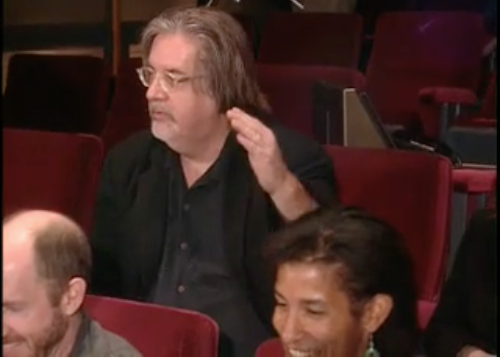
\includegraphics{images/figures/futurama_math_lecture.png} % html_ignore
\end{center}
\caption{\href{https://tauday.com/tau-manifesto/\#sec-about_the_author}{Michael Hartl} demuestra que \href{https://es.wikipedia.org/wiki/Matt_Groening}{Matt Groening} se equivoca recitando 40 dígitos decimales de $\pi$.\label{fig:futurama_video}}
\end{figure}

En verdad, las personas partidarias de $\tau$ nos enfrentamos a un imponente adversario. Y sin embargo, contamos con una poderosa aliada, pues la verdad está de nuestra parte.

% section the_most_important_number (end)

\section{El número tau} % (fold)
\label{sec:the_number_tau}

En la sección~\ref{sec:an_immodest_proposal} vimos que el número $\tau$ se puede escribir también como $2\pi$. Por tanto, como se señala en ``$\pi$ Is Wrong!'', resulta de gran interés descubrir que la combinación $2\pi$ se encuentra con asombrosa frecuencia en todas las ramas de las matemáticas. Considérense, por ejemplo, las integrales espaciales en coordenadas polares:
\[
  \int_0^{2\pi}\int_0^\infty f(r, \theta)\, r\, dr\, d\theta.
\]
El límite superior de integración de la variable $\theta$ siempre es $2\pi$. Aparece el mismo factor en la definición de la \href{https://es.wikipedia.org/wiki/Distribución_normal}{distribución gaussiana (normal)},
\[
  \frac{1}{\sqrt{2\pi}\sigma}e^{-\frac{(x-\mu)^2}{2\sigma^2}},
\]
y, nuevamente, en la  \href{http://mathworld.wolfram.com/FourierTransform.html}{transformada de Fourier},
\[
  f(x) = \int_{-\infty}^\infty F(k)\, e^{2\pi ikx}\,dk
\]
\[
    F(k) = \int_{-\infty}^\infty f(x)\, e^{-2\pi ikx}\,dx.
\]
Reaparece también en la \href{https://es.wikipedia.org/wiki/Fórmula_integral_de_Cauchy}{fórmula integral de Cauchy},
\[
  f(a) = \frac{1}{2\pi i}\oint_\gamma\frac{f(z)}{z-a}\,dz,
\]
en las $n$-ésimas \href{https://es.wikipedia.org/wiki/Raíz_de_la_unidad}{raíces de la unidad},
\[
  z^n = 1 \Rightarrow z = e^{2\pi i/n},
\]
y en los valores de la \href{https://es.wikipedia.org/wiki/Función_zeta_de_Riemann}{función zeta de Riemann} para enteros positivos pares:\footnote{Aquí $B_n$ es el $n$-ésimo \href{https://es.wikipedia.org/wiki/Número_de_Bernoulli}{número de Bernoulli}.}
\[
  \zeta(2n) = \sum_{k=1}^\infty \frac{1}{k^{2n}} = \frac{B_n}{2(2n)!}\,(2\pi)^{2n}.\qquad n = 1, 2, 3, \ldots
\]

Estas fórmulas no están cuidadosamente elegidas a propósito ---abre por cualquier página al azar tu libro favorito de física o matemáticas y compruébalo por ti mismo. Hay  \href{http://www.harremoes.dk/Peter/Undervis/Turnpage/Turnpage1.html}{muchos más ejemplos}, pero en todo caso la conclusión está clara: $2\pi$~tiene algo de peculiar.

Para llegar al fondo de este misterio, debemos volver a los principios fundamentales y analizar la naturaleza de las circunferencias, y especialmente la naturaleza de los \emph{ángulos}. Aunque es probable que la mayor parte de este material resultará familiar, merece la pena volver a pasar por él, ya que es aquí donde comienza la auténtica comprensión de $\tau$.

  \subsection{Circunferencias y ángulos} % (fold)
  \label{sec:circles_and_angles}

Existe una íntima relación entre circunferencias y ángulos, tal y como muestra la figura~\ref{fig:angle_arclength}. Como las circunferencias concéntricas en la figura~\ref{fig:angle_arclength} tienen radios diferentes, las líneas del dibujo cortan distintas \emph{longitudes de arco}, pero el ángulo~$\theta$ (theta) es el mismo en ambos casos. En otras palabras, el tamaño de los ángulos no depende del radio de la circunferencia empleada para definir el arco. La tarea principal de la medición de ángulos es crear un sistema que condense esta invarianza respecto al radio.

\begin{figure}
\begin{center}
\image{images/figures/angle-arclength.pdf}
\end{center}
\caption{Un ángulo $\theta$ con dos circunferencias concéntricas.\label{fig:angle_arclength}}
\end{figure}

Quizá el sistema de ángulos más rudimentario es el basado en  \emph{grados}, que divide una circunferencia en 360 partes iguales. Una consecuencia de este sistema es el conjunto de ángulos especiales (familiares para quienes estudian trigonometría) que muestra la figura~\ref{fig:degree_angles}.

\begin{figure}
\begin{center}
\image{images/figures/degree-angles.pdf}
\end{center}
\caption{Algunos ángulos especiales, en grados.\label{fig:degree_angles}}
\end{figure}

Existe otro sistema más fundamental de medición de ángulos que pasa por comparar directamente la longitud de arco $s$ y el radio $r$. Aunque las longitudes de la figura~\ref{fig:angle_arclength} son diferentes, la longitud de arco crece en proporción al radio, de manera que el \emph{cociente} entre la longitud de arco y el radio es el mismo en ambos casos:
\[
s\propto r \Rightarrow \frac{s_1}{r_1} = \frac{s_2}{r_2}.
\]
Esto sugiere la siguiente definición de  \emph{medida de ángulos en radianes}:
\begin{equation}
\label{eq:radians}
\theta \equiv \frac{s}{r}.
\end{equation}
Esta definición posee la propiedad requerida de ser invariante con respecto al radio, y dado que tanto  $s$ como $r$ tienen unidades de longitud, los radianes son  \href{https://es.wikipedia.org/wiki/Magnitud_adimensional}{\emph{adimensionales}} por construcción. Medir ángulos en radianes da lugar a fórmulas concisas y elegantes en matemáticas; por ejemplo, la fórmula habitual para la derivada de  $\sin\theta$ es cierta solamente cuando  $\theta$ se expresa en radianes:
\[
  \frac{d}{d\theta}\sin\theta = \cos\theta. \qquad\mbox{(cierto solo cuando $\theta$ se expresa en radianes)}
\]
Naturalmente, los ángulos especiales de la figura~\ref{fig:degree_angles} se pueden expresar en radianes, y cuando aprendiste trigonometría en secundaria probablemente tuviste que memorizar los valores especiales que se muestran en la figura~\ref{fig:pi_angles} (denomino a esta unidad de medida $\pi$-radián para enfatizar que están escritos en términos de $\pi$).

\begin{figure}
\begin{center}
\image{images/figures/pi-angles.pdf}
\end{center}
\caption{Algunos ángulos especiales, en $\pi$-radianes.\label{fig:pi_angles}}
\end{figure}

\begin{figure}
\begin{center}
\image{images/figures/angle-fractions.pdf}
\end{center}
\caption{Los ángulos ``especiales'' son fracciones de una circunferencia completa.\label{fig:angle_fractions}}
\end{figure}

Si lo pensamos por un momento, vemos que estos ángulos ``especiales'' no son más que  \emph{fracciones racionales} particularmente sencillas de una circunferencia completa, como se muestra en la figura~\ref{fig:angle_fractions}. Esto invita a revisar la ecuación~\eqref{eq:radians}, reescribiendo la longitud del arco~$s$ en función de la fracción~$f$ de la circunferencia completa~$C$, es decir, $s = f C$:
\[ \theta = \frac{s}{r} = \frac{fC}{r} =  f\left(\frac{C}{r}\right) \equiv f\tau. \]
Nótese cuán naturalmente se desprende $\tau$ de este análisis. Si eres una persona creyente en $\pi$, me temo que el diagrama  de ángulos especiales resultante (figura~\ref{fig:tau_angles}) va a sacudir tu fe desde sus entrañas.

\begin{figure}
\begin{center}
\image{images/figures/tau-angles.pdf}
\end{center}
\caption{Algunos ángulos especiales, en radianes.\label{fig:tau_angles}}
\end{figure}

Aunque hay muchos otros argumentos a favor de $\tau$, puede que la figura~\ref{fig:tau_angles} sea el más impactante. En la figura~\ref{fig:tau_angles} vemos también la genialidad de la identificación que hizo Bob Palais de la constante de la circunferencia como ``\href{https://en.wikipedia.org/wiki/Turn_(geometry)}{una vuelta}'': $\tau$ es la medida de ángulo en radianes para una \emph{vuelta} de circunferencia. Es más: nótese que con $\tau$ \emph{no hay nada que memorizar}: la duodécima parte de una vuelta es $\tau/12$, la octava parte de una vuelta es $\tau/8$, y así sucesivamente. Utilizar $\tau$ nos da lo mejor de ambos mundos, combinando claridad conceptual con todos los beneficios específicos de los radianes; el significado abstracto de, por ejemplo, $\tau/12$ es obvio, pero también es simplemente un número:
\[
  \mbox{duodécima parte de una vuelta} = \frac{\tau}{12} \approx \frac{6.283185}{12} = 0.5235988.
\]
Por último, si comparamos la figura~\ref{fig:pi_angles} con la figura~\ref{fig:tau_angles}, vemos de dónde proceden esos engorrosos factores de $2\pi$: una vuelta de circunferencia es $1\tau$, pero $2\pi$. Numéricamente son iguales, pero conceptualmente son bien distintos.

    \subsubsection{Repercusiones} % (fold)
    \label{sec:the_ramifications}
    % subsubsection the_ramifications (end)

Esos innecesarios factores de $2$ que se derivan del uso de $\pi$ son suficientemente molestos por sí mismos, pero más grave aún es su tendencia a cancelarse cuando se dividen por cualquier número par. Se producen resultados absurdos, como la  \emph{mitad} de $\pi$ para un \emph{cuarto} de vuelta, que ocultan la relación subyacente entre la medida de un angulo y la constante de la circunferencia. A quienes sostienen que ``da igual'' utilizar $\pi$ o $\tau$ al enseñar trigonometría solo les pido que traten de ver la figura~\ref{fig:pi_angles}, la figura~\ref{fig:angle_fractions} y la figura~\ref{fig:tau_angles} a través de los ojos de un niño o niña. Verán que, desde la perspectiva de quien empieza a aprender, \href{http://tauday.com/a-tau-testimonial}{\emph{usar $\pi$ en lugar de $\tau$ es un desastre pedagógico}}.
%TODO underscore not right on greek letters

  \subsection{Las funciones circulares} % (fold)
  \label{sec:the_circle_functions}

Aunque la medida de ángulos en radianes ofrece algunos de los argumentos más convincentes acerca de la constante de la circunferencia, también vale la pena comparar las virtudes de $\pi$ y $\tau$ en otros contextos. Empecemos por considerar las importantes funciones básicas $\sin\theta$ y $\cos\theta$. Conocidas como ``funciones circulares'' por dar las coordenadas de un punto en la \emph{circunferencia unitaria} (es decir, una circunferencia con radio~$1$), el seno y el coseno son funciones fundamentales en trigonometría (figura~\ref{fig:circle_functions}).

%TODO Translate figure
\begin{figure}
\begin{center}
\image{images/figures/circle-functions.pdf}
\end{center}
\caption{Las funciones circulares son coordenadas en la circunferencia unitaria.\label{fig:circle_functions}}
\end{figure}

Examinemos las gráficas de las funciones circulares para comprender mejor su comportamiento.\footnote{Estas gráficas se han generado con la ayuda de \href{http://www.wolframalpha.com/}{Wolfram|Alpha}.} En la figura ~\ref{fig:sine_with_tau} y la figura~\ref{fig:cosine_with_tau} se observa que ambas funciones son \emph{periódicas} con periodo $T$. Como se muestra en la figura~\ref{fig:sine_with_tau}, la función $\sin\theta$ comienza en cero, alcanza un máximo al llegar a un cuarto del periodo, pasa por cero en la mitad del periodo, alcanza un mínimo en las tres cuartas partes del periodo y vuelve a cero tras un periodo completo. Por su parte, la función $\cos\theta$ comienza en un máximo, tiene un mínimo en la mitad del periodo y pasa por cero en un cuarto y tres cuartos del periodo (figura~\ref{fig:cosine_with_tau}). A modo de referencia, ambas figuras muestran el valor de $\theta$ (en radianes) en cada punto especial.

%TODO Translate figure
\begin{figure}
\begin{center}
\image{images/figures/sine-with-tau.pdf}
\end{center}
\caption{Puntos importantes de $\sin\theta$ en relación con el periodo $T$.\label{fig:sine_with_tau}}
\end{figure}

\begin{figure}
\begin{center}
\image{images/figures/cosine-with-tau.pdf}
\end{center}
\caption{Puntos importantes de $\cos\theta$ en relación con el periodo $T$.\label{fig:cosine_with_tau}}
\end{figure}


Por supuesto, dado que tanto seno como coseno completan un ciclo completo tras una vuelta alrededor de la circunferencia, tenemos que $T = \tau$; es decir, las funciones circulares tienen periodos iguales a la constante de la circunferencia. Como consecuencia, los valores ``especiales''de $\theta$ son completamente naturales: un cuarto del periodo es $\tau/4$, la mitad del periodo es $\tau/2$, etc. De hecho, al generar la figura~\ref{fig:sine_with_tau}, me encontré en un momento dado pensando en cuál sería el valor numérico de $\theta$ para el cero de la función seno. Dado que el cero se produce tras medio periodo, y dado que $\tau \approx 6.28$, un cálculo mental rápido me condujo al siguiente resultado:
\[
  \theta_\mathrm{cero} = \frac{\tau}{2} \approx 3.14.
\]
Así es: me quedé atónito al descubrir que \emph{ya había olvidado que a veces $\tau/2$ se llama ``$\pi$''.} Quizá incluso te acaba de pasar lo mismo a ti.

Bienvenido o bienvenida a mi mundo.

  % subsection the_circle_functions (end)

% section radian_angle_measure (end)

   \subsection{La identidad de Euler} % (fold)
   \label{sec:euler_s_identity}

Sería un descuido por mi parte no abordar la \emph{identidad de Euler}, algunas veces calificada como ``la ecuación más hermosa de las matemáticas''. Esta identidad involucra a la \emph{exponencial compleja}, que está profundamentamente conectada tanto con la constante de la circunferencia como con su misma geometría.

Dependiendo del camino elegido, la siguiente ecuación se puede demostrar como teorema o tomar como definición; en cualquier caso, es realmente excepcional:
\begin{equation}
\label{eq:eulers_formula}
e^{i\theta} = \cos\theta + i\sin\theta. \qquad\mbox{Fórmula de Euler}
\end{equation}
%TODO Letters with accents are a bit off on mboxes
Conocida como la \emph{fórmula de Euler} (en honor a \href{https://es.wikipedia.org/wiki/Leonhard_Euler}{Leonhard Euler}), esta ecuación relaciona una exponencial con argumento imaginario con las funciones circulares seno y coseno y con la unidad imaginaria~$i$. Aunque explicar la fórmula de Euler queda fuera del alcance de este manifiesto, su origen no es precisamente sospechoso, y su importancia es incuestionable.

Evaluar la ecuación~\eqref{eq:eulers_formula} en $\theta = \tau$ da como resultado la \emph{identidad de Euler}:\footnote{Aquí estoy difiniendo implícitamente la identidad de Euler como la \emph{exponencial compleja de la constante de la circunferencia} en lugar de definirla como la exponencial compleja de cualquier número en particular. Si elegimos  $\tau$ como la constante de la circunferencia, obtenemos la identidad mostrada. Como veremos en breve, esta no es la forma tradicional de la identidad, que por supuesto involucra a $\pi$, pero la versión con  $\tau$ es la forma más  \emph{matemáticamente} significativa de la identidad, así que creo que merece el nombre.}
\[ e^{i\tau} = 1. \qquad\mbox{Identidad de Euler (versión con $\tau$)} \]
Expresada en palabras, esta ecuación realiza la siguiente observación fundamental:

\begin{center}
\emph{La exponencial compleja de la constante de la circunferencia es la unidad.}
\end{center}

Geométricamente, multiplicar por $e^{i\theta}$ equivale a rotar un número complejo un ángulo $\theta$ en el plano complejo, lo que sugiere una segunda interpretación de la identidad de Euler:

\begin{center}
\emph{Una rotación de una vuelta es 1.}
\end{center}


\noindent Dado que el número $1$ es la \href{https://es.wikipedia.org/wiki/Elemento_neutro}{identidad multiplicativa}, el significado geométrico de $e^{i\tau} = 1$ es que rotar un punto en el plano complejo una vuelta completa simplemente lo devuelve a su posición original.

Como en el caso de la medición de ángulos en radianes, vemos lo natural que resulta la asociación entre $\tau$ y una vuelta alrededor de una circunferencia. Tanto es así, que la identificación de $\tau$ con ``una vuelta'' hace que la identidad de Euler suene casi como una tautología.\footnote{Técnicamente, todos los teoremas matemáticos son tautologías, pero no seamos tan pedantes.}


    \subsubsection{No precisamente la ecuación más hermosa} % (fold)
    \label{sec:not_the_most_beautiful_equation}

Evidentemente, la forma tradicional de la ecuación de Euler se escribe en términos de $\pi$ en lugar de $\tau$. Para obtenerla, comenzamos por evaluar la fórmula de Euler en $\theta = \pi$, lo que produce
\begin{equation}
\label{eq:eulers_identity_pi}
e^{i\pi} = -1. \qquad\mbox{Identidad de Euler (versión con $\pi$)}
\end{equation}
Pero ese signo menos es tan feo que la fórmula casi siempre se reordena inmediatamente, produciendo la siguiente ``hermosa'' ecuación:
\[ e^{i\pi} + 1 = 0. \qquad\mbox{Identidad de Euler (reordenada)} \]
Al llegar a este punto, habitualmente quien explica efectúa alguna afirmación grandilocuente sobre cómo la identidad de Euler relaciona $0$, $1$, $e$, $i$ y $\pi$ ---en ocasiones llamados los ``cinco números más importantes en matemáticas''. Es impresionante la cantidad de gente que se queja de que la identidad de Euler con $\tau$ solo relaciona \emph{cuatro} de estos cinco. De acuerdo:
\[ e^{i\tau} = 1 + 0. \]
Esta fórmula, \emph{sin} reordenar, en relaciona verdaderamente los cinco números más importantes en matemáticas: $0$, $1$, $e$, $i$ y $\tau$.

      \subsubsection{Identidades eulerianas} % (fold)
      \label{sec:eulerian_identities}

Dado que es posible añadir cero en cualquier ecuación, introducir $0$ en la fórmula $e^{i\tau} = 1 + 0$ no deja de ser un contrapunto irónico a $e^{i\pi} + 1 = 0$, pero realmente puede extraerse algo importante de la identidad $e^{i\pi} = -1$. Veamos qué sucede cuando la reescribimos en términos de $\tau$:

\[
e^{i\tau/2} = -1.
\]
Geométricamente, esto significa que una rotación de media vuelta es lo mismo que multiplicar por $-1$. Y efectivamente, así es: tras una rotación de $\tau/2$ radianes, el número complejo $z = a + ib$ queda asignado a $-a - ib$, que es de hecho $-1\cdot z$.

Escrita en términos de $\tau$, vemos que la forma ``original'' de la identidad de Euler (ecuación~\eqref{eq:eulers_identity_pi}) tiene un significado geométrico obvio del que carece cuando se escribe en términos de $\pi$ (por supuesto, $e^{i\pi} = -1$ se puede interpretar como una rotación por $\pi$ radianes, pero la casi universal reordenación a la forma $e^{i\pi} + 1 = 0$ evidencia cómo el uso de $\pi$ desvía la atención del significado geométrico natural de la identidad). Las identidades de cuartos de ángulo tienen interpretaciones geométricas similares: evaluar la ecuación~\eqref{eq:eulers_formula} en $\tau/4$ nos da $e^{i\tau/4} = i$, que significa que un cuarto de vuelta en el plano complejo es lo mismo que multiplicar por~$i$; igualmente, $e^{i\cdot(3\tau/4)} = -i$ quiere decir que tres cuartos de vuelta es lo mismo que multiplicar por~$-i$. La tabla~\ref{table:eulerian_identities} presenta un resumen de estos resultados, que denominaremos \emph{identidades eulerianas}.


\begin{table}
\begin{center}
\begin{tabular}{cllr}
Ángulo de rotación & \multicolumn{3}{c}{Identidad euleriana} \\ \hline
$0$ & $e^{i\cdot0}$ & $ = $ & $1$ \smallskip \\
$\tau/4$ & $e^{i\tau/4}$ & $ = $ & $i$ \smallskip \\
$\tau/2$ & $e^{i\tau/2}$ & $ = $ & $-1$ \smallskip \\
$3\tau/4$ & $e^{i\cdot(3\tau/4)}$ & $ = $ & $-i$ \smallskip \\
$\tau$ & $e^{i\tau}$ & $ = $ & $1$
\end{tabular}
\end{center}
\caption{Identidades eulerianas para rotaciones de cuartos de vuelta, media vuelta y vuelta completa.\label{table:eulerian_identities}}
\end{table}

Podemos llevar este análisis un paso más allá señalando que, para cualquier ángulo~$\theta$, se puede interpretar $e^{i\theta}$ como un punto perteneciente a la circunferencia unidad en el plano complejo. Como el plano complejo identifica el eje horizontal con la parte real del número y el eje vertical con la parte imaginaria, la fórmula de Euler nos dice que $e^{i\theta}$ son las coordenadas $(\cos\theta, \sin\theta)$. Si introducimos los valores de los ángulos ``especiales'' de la figura~\ref{fig:tau_angles} en la ecuación~\eqref{eq:eulers_formula} obtenemos entonces los puntos de la tabla~\ref{table:complex_exponentials}, y si dibujamos estos puntos en el plano complejo obtendremos la figura~\ref{fig:tau_euler_circle}. Comparar la figura~\ref{fig:tau_euler_circle} con la figura~\ref{fig:tau_angles} disipa rápidamente cualquier duda acerca de cuál de las constantes de la circunferencia revela mejor la relación entre la fórmula de Euler y la geometría del círculo.

\begin{table}
\begin{center}
\begin{tabular}{lcc}
Forma polar & Forma rectangular & Coordenadas \\ \hline\hline
$e^{i\theta}$ & $\cos\theta + i\sin\theta$ & $(\cos\theta, \sin\theta)$ \\ \hline
$e^{i\cdot0}$ & $1$ & $(1, 0)$ \smallskip \\
$e^{i\tau/12}$ & $\frac{\sqrt{3}}{2} + \frac{1}{2}i$ & $(\frac{\sqrt{3}}{2}, \frac{1}{2})$ \smallskip \\
$e^{i\tau/8}$ & $\frac{1}{\sqrt{2}} +  \frac{1}{\sqrt{2}}i$ & $(\frac{1}{\sqrt{2}}, \frac{1}{\sqrt{2}})$ \smallskip \\
$e^{i\tau/6}$ & $\frac{1}{2} +\frac{\sqrt{3}}{2} i$ & $(\frac{1}{2}, \frac{\sqrt{3}}{2})$ \smallskip \\
$e^{i\tau/4}$ & $i$ & $(0, 1)$ \smallskip \\
$e^{i\tau/3}$ & $-\frac{1}{2} +\frac{\sqrt{3}}{2} i$ & $(-\frac{1}{2}, \frac{\sqrt{3}}{2})$ \smallskip \\
$e^{i\tau/2}$ & $-1$ & $(-1, 0)$ \smallskip \\
$e^{i\cdot(3\tau/4)}$ & $-i$ & $(0, -1)$ \smallskip \\
$e^{i\tau}$ & $1$ & $(1, 0)$
\end{tabular}
\end{center}
\caption{Exponenciales complejas de los ángulos especiales de la figura~\ref{fig:tau_angles}.\label{table:complex_exponentials}}
\end{table}

\begin{figure}
\begin{center}
\image{images/figures/tau_euler_circle.pdf}
\end{center}
\caption{Exponenciales complejas de algunos ángulos especiales dibujados en el plano complejo.\label{fig:tau_euler_circle}}
\end{figure}

      % subsubsection eulerian_identities (end)

\section{El área del círculo: el \emph{tiro de gracia}} % (fold)
\label{sec:circular_area}

Si has llegado aquí como un creyente en $\pi$, a estas alturas deberías estar cuestionando tu fe. $\tau$ es tan natural, su significado tan obvio... ¿No hay ningún ejemplo en que $\pi$ brille con toda su gloria? Se agita un recuerdo ---sí, existe una fórmula así---, ¡es la fórmula del área del círculo! Contemplad:
\[ A = \tfrac{1}{4} \pi D^2. \]
No, un momento. La fórmula del área siempre se escribe en términos del \emph{radio}, así:
\[ A = \pi r^2. \]
Aquí vemos a $\pi$, sin adornos, en una de las ecuaciones más importantes en matemáticas: una fórmula demostrada por primera vez por el mismísimo \href{https://es.wikipedia.org/wiki/Arquímedes}{Arquímedes}. ¡Queda reestablecido el orden! Y sin embargo, el nombre de esta sección suena funesto\ldots\ Si esta ecuación es la gloriosa coronación de $\pi$, ¿cómo puede ser también su \href{https://es.wikipedia.org/wiki/Tiro_de_gracia}{\emph{tiro de gracia}}?


  \subsection{Formas cuadráticas} % (fold)
  \label{sec:quadratic_forms}

Examinemos este modelo ejemplar de $\pi$, $A = \pi r^2$. Observamos que relaciona el diámetro ---no, un momento, el \emph{radio}--- elevado a la segunda potencia. Esto lo convierte en una sencilla \emph{forma cuadrática}. Tales formas se presentan en muchos contextos; como \href{http://thesis.library.caltech.edu/1940/}{físico}, mis ejemplos favoritos provienen del plan de estudios básico de la carrera de física. Vamos a considerar unos cuantos, uno detrás de otro.

    \subsubsection{Caídas en un campo gravitacional uniforme} % (fold)
    \label{sec:falling_in_a_uniform_gravitational_field}

\href{https://es.wikipedia.org/wiki/Galileo_Galilei}{Galileo Galilei} descubrió que la velocidad de un objeto que cae en un campo gravitacional uniforme es proporcional a su tiempo de caída:
\[ v \propto t. \]
La constante de proporcionalidad es la aceleración gravitacional~$g$:
\[ v = g t. \]
Como la velocidad es la derivada de la posición, podemos calcular la distancia recorrida por integración:
\[ y = \int v\,dt = \int_0^t gt\,dt = \textstyle{\frac{1}{2}} gt^2. \]


    \subsubsection{Energía potencial en un muelle lineal} % (fold)
    \label{sec:potential_energy_in_a_linear_spring}

\href{https://es.wikipedia.org/wiki/Robert_Hooke}{Robert Hooke} descubrió que la fuerza externa requerida para estirar un muelle es proporcional a su elongación:
\[ F \propto x. \]
La constante de proporcionalidad es la constante elástica del muelle~$k$:\footnote{Puede que hayas visto esto escrito como $F = -kx$. en este caso, $F$ hace referencia a la fuerza ejercida por el \emph{muelle}. Por la tercera ley de Newton, la fuerza externa de la que se habla arriba es igual y de \emph{signo opuesto} a la fuerza del muelle.}
\[ F = k x. \]
La energía potencial del muelle es por tanto igual al trabajo realizado por la fuerza externa:
\[ U = \int F\,dx = \int_0^x kx\,dx = \textstyle{\frac{1}{2}} kx^2. \]

    \subsubsection{Energía del movimiento} % (fold)
    \label{sec:energy_of_motion}

\href{https://es.wikipedia.org/wiki/Isaac_Newton}{Isaac Newton} descubrió que la fuerza ejercida sobre un objeto es proporcional a su aceleración:
\[ F \propto a. \]
La constante de proporcionalidad es la masa~$m$:
\[ F = m a. \]
La energía del movimiento, o \emph{energía cinética}, es igual al total del trabajo invertido en acelerar la masa hasta la velocidad~$v$:
\[ K = \int F\,dx = \int ma\,dx = \int m\frac{dv}{dt}\,dx = \int m\frac{dx}{dt}\,dv = \int_0^v mv\,dv = \textstyle{\frac{1}{2}} mv^2. \]

  \subsection{Un presentimiento} % (fold)
  \label{sec:a_sense_of_foreboding}

Tras haber visto varios ejemplos de formas cuadráticas simples en física, es posible que hayas sentido un presentimiento en el momento en que volvemos a la geometría de la circunferencia. Hay motivos para ello.

\begin{figure}
\begin{center}
\image{images/figures/circular-area.pdf}
\end{center}
\caption{Descomposición de un círculo en anillos.\label{fig:circular_area}}
\end{figure}

Como se puede observar en la figura~\ref{fig:circular_area}, el área de un círculo se puede calcular descomponiéndolo en anillos circulares de longitud $C$ y anchura $dr$, donde el área de cada anillo es $C\,dr$:
\[ dA = C\,dr. \]
Bien, tenemos que la circunferencia de un círculo es proporcional a su radio:
\[ C \propto r. \]
La constante de proporcionalidad es $\tau$:
\[ C = \tau\,r. \]
El área de un círculo, entonces, es la integral de todos los anillos:
\[ A = \int dA = \int_0^r C\,dr = \int_0^r \tau\,r\,dr = \textstyle{\frac{1}{2}} \tau\,r^2. \]

Si aún eras partidario acérrimo de  $\pi$ al comienzo de esta sección, ahora te ha explotado la cabeza. Y es que vemos que aún en este caso, donde supuestamente $\pi$ debía resplandecer, en realidad se ha perdido un factor de $2$. De hecho, la demostración original de Arquímedes no muestra que el área de un círculo sea $\pi r^2$, sino que es igual al área de un triángulo rectángulo de base $C$ y altura $r$. Si aplicamos la fórmula para aŕeas de triángulos obtenemos
\[
  A = \textstyle{\frac{1}{2}} bh = \textstyle{\frac{1}{2}}Cr = \textstyle{\frac{1}{2}}\tau\,r^2.
\]
Sencillamente, no hay manera de evitar ese factor de un medio (tabla~\ref{table:quadratic_forms}).

\begin{table}
\begin{center}
\begin{tabular}{lcc}
Cantidad & Símbolo & Expresión \\ \hline
Distancia en caída & $y$ & $\textstyle{\frac{1}{2}}gt^2$ \smallskip \\
Energía del muelle & $U$ & $\textstyle{\frac{1}{2}}kx^2$ \smallskip \\
Energía cinética & $K$ & $\textstyle{\frac{1}{2}}mv^2$ \smallskip \\
Área del círculo & $A$ & $\textstyle{\frac{1}{2}}\tau\,r^2$
\end{tabular}
\end{center}
\caption{Algunas formas cuadráticas habituales.\label{table:quadratic_forms}}
\end{table}

    \subsubsection{Quod erat demonstrandum} % (fold)
    \label{sec:quod_erat_demonstrandum}

En este manifiesto nos propusimos exponer que $\tau$ es la verdadera constante de la circunferencia. Dado que la fórmula del área del círculo era más o menos el último y mejor argumento que le quedaba a $\pi$ , me la voy a jugar ya mismo y voy a decir: \href{https://es.wikipedia.org/wiki/Quod_erat_demonstrandum}{Q.E.D.}

    % subsubsection quod_erat_demonstrandum (end)

% section circular_area (end)

\section{Conflicto y resistencia} % (fold)
\label{sec:conflict_and_resistance}

A pesar de esta decisiva demostración de su superioridad, hay muchas personas que se oponen a $\tau$, como notación y como número. En esta sección abordaremos las inquietudes de quienes aceptan el valor pero no la letra. Después, refutaremos algunos de los muchos argumentos reunidos contra $C/r$, incluyendo el llamado ``Manifiesto Pi'' que defiende la superioridad de $\pi$. En este contexto, discutiremos el relativamente avanzado asunto del volumen de una hiperesfera (sección~\ref{sec:volume_of_a_hypersphere}), que mejora y amplía los argumentos de la sección~\ref{sec:circular_area} sobre el área del círculo.

  \subsection{Una vuelta} % (fold)
  \label{sec:one_turn}

La verdadera prueba que debe superar cualquier notación es el uso, y después de haber visto la letra $\tau$ en uso a lo largo de todo este manifiesto, es posible que te haya convencido de que sirve bien a su propósito. Pero en el caso de una constante tan fundamental como $\tau$ estaría bien tener razones más profundas para su elección. ¿Por qué no $\alpha$, por ejemplo, u $\omega$? ¿Qué tiene $\tau$ de especial?

Hay dos razones principales para utilizar $\tau$ para representar la constante de la circunferencia. La primera es que $\tau$ se parece visualmente a $\pi$: tras siglos de uso, la asociación de $\pi$ con la constante de la circunferencia es inevitable, y el empleo de $\tau$ se nutre de esta asociación en lugar de combatirla (de hecho, la línea horizontal en ambas letras sugiere que interpretemos las ``patas'' como \emph{denominadores}, de manera que $\pi$ tiene dos patas en su denominador y $\tau$ solo una. Visto de esta forma, la relación $\tau = 2\pi$ resulta perfectamente natural).\footnote{Gracias al lector de \emph{El manifiesto tau} Jim Porter por señalar esta interpretación.}

La segunda razón es que $\tau$ se corresponde con una \emph{vuelta} (N.~del~T.: en inglés, ``turn'') alrededor de una circunferencia, y puede que hayas observado que tanto ``$\tau$'' como ``turn'' comienzan con sonido de ``\emph{t}''. Este fue el motivo original para la elección de $\tau$, y no es una coincidencia: la raíz de la palabra inglesa ``turn'' es la palabra griega τόρνος (tornos), que significa ``torno''. Si utilizamos una tipografía matemática para la primera letra de τόρνος tenemos $\tau$.

Desde la presentación original de \emph{El manifiesto tau}, he descubierto que \href{http://www.harremoes.dk/Peter/}{Peter Harremo\"{e}s} propuso de manera independiente utilizar $\tau$ a Bob Palais, autor de ``$\pi$ Is Wrong!'', en 2010, que John Fisher propuso usar $\tau$ en una \href{https://groups.google.com/forum/#!msg/sci.math/c-DHmJHSA0A/sLCoOtHB1UAJ}{publicación en Usenet} en 2004, ¡y que Joseph Lindenberg anticipó tanto la discusión como el símbolo más de veinte años antes (Lindenberg ha colgado tanto su manuscrito original a máquina como un gran número de argumentos en su página web \href{http://sites.google.com/site/taubeforeitwascool/}{Tau Before It Was Cool})! El Dr.~Harremo\"{e}s ha destacado la importancia de un aspecto ya presentado en la sección~\ref{sec:an_immodest_proposal}: emplear $\tau$ da un \emph{nombre} a la constante de la circunferencia. Dado que $\tau$ es una letra griega común, aquellas personas que la encuentren por primera vez pueden pronunciarla inmediatamente. Más aún, a diferencia de llamar a la constante de la circunferencia ``una vuelta'',
$\tau$ funciona bien tanto en contextos escritos como orales. Por ejemplo, decir que el ángulo de un cuarto de circunferencia en radianes es ``un cuarto de vuelta'' en radianes suena muy bien, pero ``vuelta cuartos radianes'' suena forzado, y ``el área de un círculo es media vuelta por $r$ al cuadrado'' suena realmente raro. Utilizando $\tau$, podemos decir ``tau cuartos radianes'' y ``el área de un círculo es tau medios por $r$ al cuadrado''.

    \subsubsection{Notación ambigua} % (fold)
    \label{sec:ambiguous_notation}

No hay duda de que cualquier notación nueva conlleva un potencial conflicto con el uso preexistente. Como se señala en la sección~\ref{sec:an_immodest_proposal}, ``$\pi$ Is Wrong!''\ evita este problema acuñando un nuevo símbolo (figura~\ref{fig:palais_tau}). Existen precedentes de esta práctica; por ejemplo, en los primeros tiempos de la mecánica cuántica \href{https://es.wikipedia.org/wiki/Max_Planck}{Max Planck} introdujo la constante~$h$, que relaciona la energía de una partícula de luz con su energía (de la forma $E = h\nu$), pero el mundo de la física pronto se dio cuenta de que a menudo resultaba más cómodo utilizar $\hbar$ (léase ``hache barra'') ---donde $\hbar$ simplemente es $h$ dividido entre\ldots\ hum\ldots\ $2\pi$--- y su uso es ahora estándar. No obstante, es difícil lograr la aceptación de un nuevo símbolo: debe dársele un nombre, se debe popularizar y el símbolo en sí debe añadirse a los sistemas de procesamiento de textos y tipografías. Por otra parte, promulgar un nuevo símbolo para $2\pi$ requeriría la cooperación de la comunidad académica matemática, que en la cuestión de $\pi$ vs.\ $\tau$ ha sido hasta el momento apática en el mejor de los casos y hostil en el peor. Emplear un símbolo que ya existe nos facilitará brujulear dentro del establishment matemático (quizá algún día la comunidad matemática consensuará un símbolo diferente para $2\pi$; si eso llega a suceder, me reservo el derecho de apoyar su propuesta. Pero han tenido más de trescientos años para arreglar este problema en torno a $\pi$, así que yo esperaría sentado).

Antes que promover un símbolo nuevo, \emph{El manifiesto tau} opta por el uso de una letra griega existente. Por ello, dado que $\tau$ ya se utiliza en algunos contextos, debemos atender a los conflictos con la práctica vigente. Por suerte hay sorprendentemente pocos usos comunes. Aún más, aunque $\tau$ se utiliza para ciertas variables \emph{específicas} ---por ejemplo, \emph{tensión cortante} en ingeniería mecánica, \emph{torque} en mecánica rotacional y  \emph{tiempo propio} en relatividad especial y general--- no hay ningún uso conflictivo \emph{universal}.\footnote{Posiblemente la única excepción sea la \emph{proporción áurea}, que normalmente se denota mediante $\tau$ en Europa. Pero además de existir una alternativa común a esta notación ---a saber, la letra griega $\varphi$---, este uso demuestra que existe un precedente para asignar $\tau$ a una constante matemática fundamental.} En estos casos, podemos tolerar la ambigüedad o evitar los escasos conflictos existentes cambiando de manera selectiva la notación, usando por ejemplo $N$ para el torque\footnote{Esta alternativa para el torque ya se utiliza; véase, por ejemplo, \emph{Introduction to Electrodynamics} de David Griffiths, p.~162.} o $\tau_p$ para el tiempo propio.

A pesar de estos argumentos, los potenciales usos conflictivos han sido la mayor fuente de oposición a $\tau$. Algunos periodistas han llegado a negar categóricamente que $\tau$ (o, presumiblemente, cualquier otro símbolo actualmente en uso) pudiera superar estos problemas. Pero la ciencia y la ingeniería tienen una elevada tolerancia a la ambigüedad notacional, y afirmar que $\tau$ como constante de la circunferencia no puede coexistir con otros usos ignora la existencia de una significativa evidencia en sentido contrario.

Un ejemplo de  ambigüedad que se tolera tranquilamente se da en mecánica cuántica, donde encontramos la siguiente fórmula para el  \emph{radio de Bohr}, que (\textit{grosso modo}) es el ``tamaño'' de un átomo de hidrógeno en su estado de mínima energía (el \emph{estado fundamental}):
\[
a_0 = \frac{\hbar^2}{m e^2},
\]
donde $m$ es la masa del electrón y $e$ es su carga. Por su parte, el estado fundamental en sí mismo se describe mediante una cantidad conocida como la \href{https://es.wikipedia.org/wiki/Función_de_onda}{\emph{función de onda}}, que decae exponencialmente con el radio en una escala de longitud establecida por el radio de Bohr:

\begin{equation}
\label{eq:hydrogen}
\psi(r) = N\,e^{-r/a_0},
\end{equation}
donde $N$ es una constante de normalización.

¿Ya te has dado cuenta del problema? Probablemente no, y ese es precisamente el asunto. El ``problema'' es que la $e$ en el radio de Bohr y la $e$ en la función de onda \emph{no son la misma $e$} ---la primera es la carga del electrón, mientras que la segunda es el número de Euler (la base de los logaritmos naturales). De hecho, si desarrollamos el factor $a_0$ en el exponente en la ecuación~\eqref{eq:hydrogen}, obtenemos
\[
\psi(r) = N\,e^{-m e^2 r/\hbar^2},
\]
que tiene una $e$ elevado a algo que contiene otra $e$ distinta. Es aún peor de lo que parece, porque la propia $N$ también contiene a $e$:
\[
\psi(r) = \sqrt{\frac{1}{\pi a_0^3}}\,e^{-r/a_0} =\frac{m^{3/2} e^3}{\pi^{1/2} \hbar^3}\,e^{-m e^2 r/\hbar^2}.
\]

No me cabe ninguna duda de que si no hubiera existido una notación específica para el número de Euler, a cualquier persona que hubiera propuesto la letra $e$ se le habría dicho que era imposible por entrar en conflicto con otros usos. Y a pesar de ello, en la práctica nadie ha tenido nunca ningún problema en usar $e$ en los dos contextos arriba señalados. Hay muchos otros ejemplos, que incluyen situaciones donde incluso $\pi$ se utiliza para dos cosas distintas.\footnote{Véase, por ejemplo, \emph{An Introduction to Quantum Field Theory} de Peskin y Schroeder, donde $\pi$ se utiliza tanto para denotar la constante de la circunferencia como para un ``momento conjugado'' en la misma página (p.~282).} Resulta difícil explicar por qué utilizar $\tau$ para distintos números es diferente.

Por cierto, los pedantes de $\pi$ que hay por ahí (y está demostrado que hay muchos) podrían señalar que la función de onda del estado fundamental del hidrógeno tiene un factor de $\pi$:
\[
\psi(r) = \sqrt{\frac{1}{\pi a_0^3}}\,e^{-r/a_0}.
\]
A simple vista, esta forma parece más natural que la versión con $\tau$:
\[
\psi(r) = \sqrt{\frac{2}{\tau a_0^3}}\,e^{-r/a_0}.
\]
Pero como de costumbre, las apariencias engañan: el valor de $N$ procede del producto
\[
\frac{1}{\sqrt{2\pi}} \frac{1}{\sqrt{2}} \frac{2}{a_0^{3/2}},
\]
que muestra que la constante de la circunferencia entra en el cálculo mediante la expresión $1/\sqrt{2\pi}$, es decir, $1/\sqrt{\tau}$. Como en la fórmula del área del círculo, que la cancelación deje un $\pi$ desnudo es mera coincidencia.

    % subsubsection ambiguous_notation (end)


  \subsection{El manifiesto pi} % (fold)
  \label{sec:the_pi_manifesto_a_rebuttal}

Aunque la mayoría de la objecciones a $\tau$ proceden de correspondencia dispersa por correo electrónico y comentarios variados en la web, también hay una resistencia organizada. En concreto, tras la publicación de \emph{El manifiesto tau} en junio de 2010 ha aparecido un ``\href{http://www.thepimanifesto.com/}{Manifesto pi}'' para defender la constante de la circunferencia tradicional. Esta sección y las dos siguientes contienen una réplica de sus razonamientos. Necesariamente, su tratamiento es más escueto y avanzado que el resto del manifiesto, pero incluso una lectura superficial de lo que sigue da una idea de la debilidad de los argumentos de El manifiesto pi.

Aunque ciertamente podemos considerar la aparición de El manifiesto pi como un signo positivo de interés continuado en este asunto, hace bastantes afirmaciones falsas. Por ejemplo, alega que el factor de $2\pi$ en la distribución gaussiana (normal) es una coincidencia, y que puede escribirse de manera más natural como
\[
\frac{1}{\sqrt\pi(\sqrt 2\sigma)}e^{\frac{-x^2}{(\sqrt 2\sigma)^2}}.
\]

Esto es falso: el factor de $2\pi$ proviene de elevar al cuadrado la distribución gaussiana no normalizada y cambiar a coordenadas polares, lo que conduce a un factor de $1$ de la integral radial y  $2\pi$ de la integral angular. Como en el caso del área del círculo, el factor de $\pi$ proviene de $1/2\times 2\pi$, no de $\pi$ solo.

Una afirmación relacionada es que la \href{http://mathworld.wolfram.com/GammaFunction.html}{función gamma} evaluada en $1/2$ es más natural en términos de $\pi$:
\[
\Gamma(\textstyle{\frac{1}{2}}) = \sqrt{\pi},
\]
donde
\begin{equation}
\label{eq:gamma}
\Gamma(p) = \int_{0}^{\infty} x^{p-1} e^{-x}\,dx.
\end{equation}
Pero $\Gamma(\frac{1}{2})$ se reduce a la misma integral gaussiana que en la distribución normal (tras establecer $u = x^{1/2}$), así que $\pi$ en este caso es también en realidad $1/2\times 2\pi$. De hecho, en muchos de los casos que se citan en El manifiesto pi la constante de la circunferencia aparece mediante una integral en que $\theta$ varía de $0$ a $\tau$.

El manifiesto pi también considera algunas fórmulas de polígonos regulares de
$n$ lados (o ``$n$-ágonos''). Por ejemplo, señala que la suma de los ángulos internos de un $n$-ágono viene dada por
\[
\sum_{i=1}^n \theta_i=(n-2)\pi.
\]
Esta cuestión fue tratada en ``Pi Is Wrong!'', que señala lo siguiente: ``la suma de los ángulos interiores [de un triángulo] es $\pi$, de acuerdo. Pero la suma de los ángulos \emph{exteriores} de \emph{cualquier} polígono, de la que la suma de los ángulos interiores se puede derivar fácilmente, y que se generaliza como la integral de la curvatura de una curva cerrada simple, es $2\pi$''. Además, El manifiesto pi presenta la fórmula del área de un $n$-ágono con radio (la distancia desde el centro hasta un vértice) unidad,
\[ A=n\sin\frac{\pi}{n}\cos\frac{\pi}{n}, \]
que presenta como ``claramente\ldots\ otra victoria para $\pi$''. Pero si utilizamos la identidad del ángulo doble $\sin\theta\cos\theta = \frac{1}{2} \sin 2\theta$ vemos que esa expresión se puede reescribir como
\[ A = n/2\, \sin\frac{2\pi}{n}, \]
que no es más que
\begin{equation}
\label{eq:area_polygon}
A = \frac{1}{2} n\, \sin\frac{\tau}{n}.
\end{equation}
En otras palabras, el área de un $n$-ágono tiene de forma natural un factor de $1/2$. De hecho, tomar el límite de la ecuación~\eqref{eq:area_polygon} cuando $n\rightarrow \infty$ (y aplicar la \href{http://mathworld.wolfram.com/LHospitalsRule.html}{regla de l'H\^{o}pital}) proporciona el área de un polígono regular unitario con infinitos lados, es decir, una circunferencia unitaria:
\begin{equation}
\label{eq:lhopital}
A = \lim_{n\rightarrow\infty} \frac{1}{2} n\, \sin\frac{\tau}{n}
= \frac{1}{2} \lim_{n\rightarrow\infty} \frac{\sin\frac{\tau}{n}}{1/n} = \tfrac{1}{2}\tau.
\end{equation}

A este respecto, debemos mencionar que El manifiesto pi arma mucho revuelo con que $\pi$ es el área de un círculo unitario, de manera que (por ejemplo) el área de un cuarto de círculo (unitario) es $\pi/4$. Esto, se afirma, arguye a favor de $\pi$ tanto como la medición de ángulos en radianes lo hace por $\tau$. Por desgracia para este argumento, como se señala en la sección~\ref{sec:circular_area} y como hemos visto de nuevo en la ecuación~\eqref{eq:lhopital}, el factor de $1/2$ surge naturalmente en el contexto del área del círculo. De hecho, la fórmula para el área de un sector circular que subtiende un ángulo~$\theta$ es

\[
\tfrac{1}{2}\theta\, r^2,
\]
así que, en general, no hay manera de evitar el factor de $1/2$ (vemos por tanto que $A = \frac{1}{2} \tau\, r^2$ es simplemente un caso especial en que  $\theta = \tau$).

En resumen, la distinción entre la medición de ángulos y de áreas no es arbitraria. No hay un factor natural de $1/2$ en el caso de la medición de ángulos. En cambio, en el caso del área el factor de $1/2$ surge de la integral de una función lineal asociada a una mera forma cuadrática. De hecho, los argumentos a favor de $\pi$ lo tienen aún peor de lo que parece, como se muestra en la siguiente sección.

  % subsection the_pi_manifesto_a_rebuttal (end)

\section{El fondo de la cuestión de pi y tau} % (fold)
\label{sec:getting_to_the_bottom_of_pi}

Aún me impresiona lo rico que es este asunto, y mi comprensión de $\pi$ y $\tau$ continúa madurando. En el día de la mitad de tau de 2012, creo que comprendí \emph{exactamente} cuál es el problema de $\pi$. Mis razonamientos pivotaban sobre un análisis del área de la superficie y el volumen de una esfera de $n$ dimensiones, que (como se muestra más abajo) evidencia que $\pi$ no tiene ningún significado geométrico fundamental. Sin embargo, mi análisis estaba incompleto, hecho del que me advirtió un extraordinario mensaje de Jeff Cornell, lector de \emph{El manifiesto tau}. En consecuencia, esta sección es un intento no solo de desenmascarar a $\pi$ definitivamente, sino también de explicar la verdad sobre $\tau$, una verdad que es más profunda y sutil de lo que me había imaginado.

\emph{Nota}: esta sección es más complicada que el resto del manifiesto y se puede saltar sin pérdida de continuidad. Si te resulta confusa, te recomiendo que pases directamente a las conclusiones en la sección~\ref{sec:conclusion}.

  \subsection{Área superficial y volumen de una hiperesfera} % (fold)
  \label{sec:volume_of_a_hypersphere}

Comencemos nuestro estudio generalizando una circunferencia a un número arbitrario de dimensiones.\footnote{Esta discusión se basa en \href{http://spikedmath.com/forum/viewtopic.php?f=30&t=147\#p1577}{una excelente observación de John Kodegadulo} en \href{http://spikedmath.com/}{spikedmath.com}.} Este objeto, llamado \emph{hiperesfera} o \emph{$n$-esfera}, se puede definir de la siguiente manera\footnote{Geómetras y topólogos/as emplean \href{http://mathworld.wolfram.com/Hypersphere.html}{definiciones de hiperesferas incompatibles}; este análisis utiliza las definiciones de los/as geómetras.} (por comodidad, asumimos que estas esferas están centradas en el origen). Una $0$-esfera es el conjunto vacío, y definimos su ``interior'' como un punto.\footnote{Esto tiene sentido, porque un punto no tiene límites,  es decir, los límites de un punto son el conjunto vacío.} Una $1$-esfera es el conjunto de todos los puntos que satisfacen
\[
x^2 = r^2,
\]
que consiste en el par de puntos $\pm r$. Su interior, que satisface
\[
x^2 \leq r^2,
\]
es el segmento que une $-r$ con $r$. Una $2$-esfera es una circunferencia, que es el conjunto de todos los puntos que satisfacen
\[
x^2 + y^2 = r^2.
\]
Su interior, que satisface
\[
x^2 + y^2 \leq r^2,
\]
es un círculo. De manera similar, una $3$-esfera satisface
\[
x^2 + y^2 + z^2 = r^2,
\]
y su interior es una esfera. La generalización a un $n$ arbitrario, aunque resulta difícil de visualizar para $n > 3$, es sencilla: una $n$-esfera es el conjunto de todos los puntos que satisfacen
\[
\sum_{i=1}^{n} x_i^2 = r^2.
\]

El manifiesto pi (tratado en la sección~\ref{sec:the_pi_manifesto_a_rebuttal}) proporciona cierta fórmula para el volumen de una $n$-esfera unitaria como un argumento a favor de $\pi$:
\begin{equation}
\label{eq:unit_n_sphere_pi}
\frac{\sqrt{\pi}^{n} }{\Gamma(1 + \frac{n}{2})},
\end{equation}
donde la función gamma viene dada por la ecuación~\eqref{eq:gamma}. La ecuación~\eqref{eq:unit_n_sphere_pi} es un caso especial de la fórmula para un radio cualquiera, que típicamente se escribe también en términos de $\pi$:
\begin{equation}
\label{eq:n_sphere_pi}
V_n(r) = \frac{\pi^{n/2} r^n}{\Gamma(1 + \frac{n}{2})}.
\end{equation}
Como $V_n(r) = \int S_n(r)\,dr$, tenemos que $S_n(r) = dV_n(r)/dr$, lo que significa que el área superficial se puede expresar de la siguiente manera:
\begin{equation}
\label{eq:n_sphere_pi_r}
S_n(r) = \frac{n \pi^{n/2} r^{n-1}}{\Gamma(1 + \frac{n}{2})}.
\end{equation}
En lugar de quedarnos con estas fórmulas tal cual, veamos si podemos desenmarañarlas para arrojar un poco más de luz sobre la cuestión de $\pi$ vs. $\tau$. Comencemos nuestro análisis señalando que su aparente simplicidad es una ilusión: aunque la función gamma es notacionalmente sencilla, se trata de hecho de una integral sobre un dominio semi-infinito, que no es una idea en absoluto sencilla. Por suerte, la función gamma se puede simplificar en ciertos casos especiales. Por ejemplo, cuando $n$ es un entero, es fácil demostrar (integrando por partes) que
\[
\Gamma(n) = (n-1)(n-2)\ldots 2\cdot 1 = (n-1)!
\]
Vista de esta manera, $\Gamma$ se puede interpretar como una generalización de la función factorial en el dominio de los números reales.\footnote{De hecho, la generalización en el dominio de los números complejos es inmediata: basta con reemplazar una $x$ real por una  $z$ compleja en la ecuación~\eqref{eq:gamma}.}

En las fórmulas de las áreas superficiales y los volúmenes de $n$ dimensiones, el argumento de $\Gamma$ no es necesariamente un entero, sino que tiene la forma $\left(1 + \frac{n}{2}\right)$, que es un entero cuando $n$ es par y un número \emph{semientero} cuando $n$ es impar. Si tomamos esto en cuenta obtenemos la siguiente expresión, que está tomada de una referencia estándar, \href{http://mathworld.wolfram.com/Hypersphere.html}{Wolfram MathWorld}, y, como es habitual, se encuentra escrita en términos de~$\pi$:
\begin{equation}
\label{eq:surface_area_mathworld}
S_n(r) = \begin{cases}
\displaystyle \frac{2\pi^{n/2}\,r^{n-1}}{(\frac{1}{2}n - 1)!} & \text{si } n \text{ es par}; \\ \\
 \displaystyle \frac{2^{(n+1)/2}\pi^{(n-1)/2}\,r^{n-1}}{(n-2)!!} & \text{si } n \text{ es impar}.
\end{cases}
\end{equation}

Integrando respecto a $r$ tenemos
\begin{equation}
\label{eq:volume_mathworld}
V_n(r) = \begin{cases}
\displaystyle \frac{\pi^{n/2}\,r^n}{(\frac{n}{2})!} & \text{si } n \text{ es par}; \\ \\
\displaystyle \frac{2^{(n+1)/2}\pi^{(n-1)/2}\,r^n}{n!!} & \text{si } n \text{ es impar}.
\end{cases}
\end{equation}

Examinemos la ecuación ~\eqref{eq:volume_mathworld} en detalle. Notése en primer lugar que MathWorld utiliza la \emph{función doble factorial}~$n!!$ ---pero, curiosamente, solo la utiliza en el caso \emph{impar} (una pista de lo que se avecina). La función doble factorial, aunque raramente se encuentra en matemáticas, es elemental: es como la función factorial normal, pero sustrayendo $2$ en cada paso en lugar de $1$, de manera que, por ejemplo, $5!! = 5 \cdot 3 \cdot 1$ y $6!! = 6 \cdot 4 \cdot 2$. En general, tenemos
\begin{equation}
\label{eq:double_factorial}
n!! = \begin{cases}
n(n-2)(n-4)\ldots6\cdot4\cdot2 & \text{si } n \text{ es par}; \\ \\
n(n-2)(n-4)\ldots5\cdot3\cdot1 & \text{si } n \text{ es impar}.
\end{cases}
\end{equation}
(por definición, $0!! = 1!! = 1$). Nótese que la ecuación~\eqref{eq:double_factorial} se divide naturalmente entre casos pares e impares, lo que torna en aún más extraña la decisión de MathWorld de utilizarla solo en el caso impar.

Para resolver este misterio, empecemos por examinar más de cerca la fórmula para $n$ impar de la ecuación~\eqref{eq:volume_mathworld}:
\[ \frac{2^{(n+1)/2}\pi^{(n-1)/2}\,r^n}{n!!} \]
Tras examinar la expresión
\[ 2^{(n+1)/2}\pi^{(n-1)/2}, \]
nos damos cuenta de que puede reescribirse como
\[ 2(2\pi)^{(n-1)/2}, \]
y aquí encontramos de nuevo a nuestro viejo amigo~$2\pi$.

Veamos ahora el caso par de la ecuación~\eqref{eq:volume_mathworld}. Hemos señalado más arriba lo raro que resulta usar la factorial ordinaria en el caso par pero la doble factorial en el impar. De hecho, como la doble factorial ya está definida a trozos, si unificamos las fórmulas utilizando $n!!$ en ambos casos podemos sacarla como factor común:
\[
V_n(r) = \frac{1}{n!!}\times \begin{cases}
\ldots & \text{si } n \text{ es par}; \\ \\
 \ldots & \text{si } n \text{ es impar}.
 \end{cases}
\]
Bien, ¿hay alguna conexión entre la función factorial y la doble factorial? Sí: cuando $n$ es par, se relacionan mediante la siguiente identidad:
\[ \left(\frac{n}{2}\right)! = \frac{n!!}{2^{n/2}} \]
(esto es fácil de verificar por \href{https://es.wikipedia.org/wiki/Inducción_matemática}{inducción}). Sustituyendo en la fórmula del volumen para $n$ par tenemos
\[ \frac{2^{n/2}\pi^{n/2}\,r^n}{n!!}, \]
que guarda un parecido notable con
\[ \frac{(2\pi)^{n/2}\,r^n}{n!!}, \]
y encontramos de nuevo un factor $2\pi$.

Uniendo estos resultados, vemos que la ecuación~\eqref{eq:volume_mathworld} se puede reescribir como
\begin{equation}
\label{eq:volume_2pi}
V_n(r) = \begin{cases}
 \displaystyle \frac{(2\pi)^{n/2}\,r^n}{n!!} & \text{si } n \text{ es par}; \\ \\
 \displaystyle \frac{2(2\pi)^{(n-1)/2}\,r^n}{n!!} & \text{si } n \text{ es impar}
 \end{cases}
\end{equation}
y la ecuación~\eqref{eq:surface_area_mathworld} se puede reescribir como
\begin{equation}
\label{eq:surface_area_2pi}
S_n(r) = \begin{cases}
\displaystyle \frac{(2\pi)^{n/2}\,r^{n-1}}{(n-2)!!} & \text{si } n \text{ es par}; \\ \\
\displaystyle \frac{2(2\pi)^{(n-1)/2}\,r^{n-1}}{(n-2)!!} & \text{if } n \text{ es impar.}
\end{cases}
\end{equation}

Sustituyendo $\tau=2\pi$ en la ecuación~\eqref{eq:surface_area_2pi} obtenemos
\[
S_n(r) = \begin{cases}
\displaystyle \frac{\tau^{n/2}\,r^{n-1}}{(n-2)!!} & \text{si } n \text{ es par}; \\ \\
\displaystyle \frac{2\tau^{(n-1)/2}\,r^{n-1}}{(n-2)!!} & \text{si } n \text{ es impar.}
\end{cases} \]
Para unificar aún más estas fórmulas, podemos utilizar la \emph{función suelo} $\lfloor x \rfloor$, que es simplemente el mayor entero menor o igual que $x$ (es equivalente a eliminar la parte fraccional, de manera que, por ejemplo, $\lfloor 3.7 \rfloor = \lfloor 3.2 \rfloor = 3$). Esto nos da
\[ S_n(r) = \begin{cases}
 \displaystyle \frac{\tau^{\left\lfloor \frac{n}{2} \right\rfloor}\,r^{n-1}}{(n-2)!!} & \text{si } n \text{ es par}; \\ \\
 \displaystyle \frac{2\tau^{\left\lfloor \frac{n}{2} \right\rfloor}\,r^{n-1}}{(n-2)!!} & \text{si } n \text{ es impar},
 \end{cases} \]
lo que nos permite escribir la fórmula de la siguiente manera:
\begin{equation}
\label{eq:surface_area_tau}
S_n(r) = \frac{\tau^{\left\lfloor \frac{n}{2} \right\rfloor}\,r^{n-1}}{(n-2)!!}\times \begin{cases}
1 & \text{si } n \text{ es par}; \\ \\
2 & \text{si } n \text{ es impar}.
\end{cases}
\end{equation}
Por último, integrar la ecuación~\eqref{eq:surface_area_tau} respecto a $r$ nos da la expresión:
\begin{equation}
\label{eq:volume_tau}
V_n(r) = \frac{\tau^{\left\lfloor \frac{n}{2} \right\rfloor}\,r^n}{n!!}\times \begin{cases}
1 & \text{si } n \text{ es par}; \\ \\
2 & \text{si } n \text{ es impar}.
\end{cases}
\end{equation}

\subsubsection{Lambda} % (fold)
\label{sec:lambda}

Las fórmulas en las ecuaciones~\eqref{eq:surface_area_tau} y~\eqref{eq:volume_tau} suponen una considerable mejora respecto a las formulaciones originales (las ecuaciones~\eqref{eq:surface_area_mathworld} y~\eqref{eq:volume_mathworld}) en términos de $\pi$. Pero en realidad resulta posible una simplificación adicional, utilizando para ello la medida de un \emph{ángulo recto}:\footnote{Jeff Cornell sugirió este cambio de notación y el análisis general.}
\begin{equation}
\label{eq:lambda}
\lambda = \frac{\tau}{4}.
\end{equation}
Como veremos en la sección~\ref{sec:three_families_of_constants}, la ecuación~\eqref{eq:lambda} se puede reescribir de forma más natural en términos de las simetrías de la circunferencia:
\begin{equation}
\label{eq:tau_lambda}
\tau = 2^2 \lambda,
\end{equation}
donde el factor de $2^2$ proviene de los $2^2$ arcos circulares congruentes (uno en cada cuadrante) en el espacio de dos dimensiones.

La mayor ventaja de $\lambda$ es que unifica completamente los casos par e impar en las ecuaciones~\eqref{eq:surface_area_tau} y~\eqref{eq:volume_tau}, cada una de las cuales tiene un factor de $\tau^{\left\lfloor \frac{n}{2} \right\rfloor}$. Efectuando la sustitución de la ecuación~\eqref{eq:tau_lambda} obtenemos
\[
\tau^{\left\lfloor \frac{n}{2} \right\rfloor} = (2^2\lambda)^{\left\lfloor \frac{n}{2} \right\rfloor} = 2^{2\left\lfloor \frac{n}{2} \right\rfloor} \lambda^{\left\lfloor \frac{n}{2} \right\rfloor} =
\lambda^{\left\lfloor \frac{n}{2} \right\rfloor}\times
\begin{cases}
 2^n & \text{si } n \text{ es par}; \\ \\
 2^{n-1} & \text{si } n \text{ es impar}.
 \end{cases}
\]
Esto significa que podemos reescribir el producto
\[
\tau^{\left\lfloor \frac{n}{2} \right\rfloor}\times \begin{cases}
1 & \text{si } n \text{ es par}; \\ \\
2 & \text{si } n \text{ es impar}.
\end{cases}
\]
como
\begin{equation}
\label{eq:prefactor}
\lambda^{\left\lfloor \frac{n}{2} \right\rfloor} \times
\begin{cases}
 2^n & \text{si } n \text{ es par}; \\ \\
 2^{n-1} & \text{si } n \text{ es impar}.
 \end{cases}
  \times \begin{cases}
 1 & \text{si } n \text{ es par}; \\ \\
 2 & \text{si } n \text{ es impar}.
 \end{cases}
 = 2^n\,\lambda^{\left\lfloor \frac{n}{2} \right\rfloor},
\end{equation}
lo que elimina la dependencia explícita de la \href{https://es.wikipedia.org/wiki/Números_pares_e_impares}{paridad}. Aplicando la ecuación~\eqref{eq:prefactor} a la ecuación~\eqref{eq:surface_area_tau} y a la ecuación~\eqref{eq:volume_tau}, tenemos que
\begin{equation}
\label{eq:surface_area_lambda}
S_n(r) = \frac{2^n\,\lambda^{\left\lfloor \frac{n}{2} \right\rfloor}\,r^{n-1}}{(n-2)!!}
\end{equation}
y
\begin{equation}
\label{eq:volume_lambda}
V_n(r) = \frac{2^n\,\lambda^{\left\lfloor \frac{n}{2} \right\rfloor}\,r^n}{n!!}.
\end{equation}

Puede parecer que las simplificaciones en las ecuaciones~\eqref{eq:surface_area_lambda} y~\eqref{eq:volume_lambda} aparecen a costa de introducir un factor de $2^n$, pero aun esto tiene un significado geométrico claro: una esfera en $n$ dimensiones se divide naturalmente en $2^n$ partes congruentes, que se corresponden con las $2^n$ familias de soluciones de $\sum_{i=1}^{n} x_i^2 = r^2$ (una para cada posible elección de $\pm x_i$). En dos dimensiones, existen los arcos para cada uno de los cuatro cuadrantes; en tres dimensiones, tenemos los sectores de esfera en cada octante; y así sucesivamente en dimensiones superiores. En otras palabras, podemos aprovechar la simetría de la esfera para calcular el área superficial o el volumen de \emph{una} parte ---típicamente la \emph{parte principal} en que $x_i > 0$ para cada $i$--- y hallar entonces el valor completo multiplicando por~$2^n$.


Hasta donde sé, las ecuaciones~\eqref{eq:surface_area_lambda} y~\eqref{eq:volume_lambda} son las formulaciones más sencillas posibles de las fórmulas para la superficie y el volumen de esferas (de hecho son las únicas que he sido capaz de memorizar fiablemente). Consideremos en particular la fórmula del volumen: a diferencia de la  \emph{falsa} simplicidad de la ecuación~\eqref{eq:n_sphere_pi}, la ecuación~\eqref{eq:volume_lambda} no involucra ninguna integral sofisticada ---tan solo las ligeramente exóticas pero en todo caso elementales funciones suelo y doble factorial. El volumen de una $n$-esfera unitaria es simplemente el volumen de cada parte simétrica, $\lambda^{\left\lfloor \frac{n}{2} \right\rfloor}/n!!$, multiplicado por el número de partes, $2^n$.

% subsubsection lambda (end)


\subsubsection{Relaciones de recurrencia} % (fold)
\label{sec:recurrences}

Ya hemos visto, en las ecuaciones~\eqref{eq:surface_area_lambda} y~\eqref{eq:volume_lambda}, que las fórmulas del área superficial y el volumen se expresan de la manera más sencilla posible en términos del ángulo recto~$\lambda$. Sin embargo, aún no hemos acabado con $\tau$.

Como ilustra la ecuación~\eqref{eq:volume_lambda}, la fórmula del volumen se divide naturalmente en dos familias, que se corresponden con espacios con número de dimensiones pares e impares, respectivamente. Esto significa que el volumen de cuatro dimensiones, $V_4$, se relaciona fácilmente $V_2$ pero no con $V_3$, mientras que $V_3$ se relaciona con $V_1$ pero no con $V_2$. ¿Cómo se relacionan exactamente?

Podemos encontrar la respuesta a esta pregunta hallando las \emph{relaciones de recurrencia} entre dimensiones.\footnote{El artículo ``\href{http://www2.math.uconn.edu/~mariano/research/MathClubsp14\%20.pdf}{The volume of the unit ball in \emph{n} dimensions}'' de Phanuel A. Mariano contiene una derivación alternativa de estas importantes relaciones de recurrencia.} En particular, dividamos el volumen de una esfera de $n$ dimensiones por el volumen de una esfera de $(n-2)$ dimensiones:
\begin{equation}
\label{eq:volume_recurrence}
\frac{V_n(r)}{V_{n-2}(r)} =
\frac{2^n}{2^{n-2}}
\frac{\lambda^{\left\lfloor \frac{n}{2} \right\rfloor}}{\lambda^{\left\lfloor \frac{n-2}{2} \right\rfloor}}
\frac{(n-2)!!}{n!!}
\frac{r^{n}}{r^{n-2}}
=
\frac{2^2\lambda}{n}\,r^2.
\end{equation}
Vemos en la ecuación~\eqref{eq:volume_recurrence} que podemos obtener el volumen de una $n$-esfera simplemente multiplicando la fórmula para una $(n-2)$-esfera por $r^2$ (un factor que exige el análisis dimensional), dividiendo por $n$ y multiplicando por la ``constante de recurrencia'' $2^2\lambda$.

De manera similar, para el área superficial tenemos que
\begin{equation}
\label{eq:surface_area_recurrence}
\frac{S_n(r)}{S_{n-2}(r)} =
\frac{2^n}{2^{n-2}}
\frac{\lambda^{\left\lfloor \frac{n}{2} \right\rfloor}}{\lambda^{\left\lfloor \frac{n-2}{2} \right\rfloor}}
\frac{(n-2-2)!!}{(n-2)!!}
\frac{r^{n}}{r^{n-2}}
=
\frac{2^2\lambda}{n-2}\,r^2,
\end{equation}
con la misma constante de recurrencia $2^2\lambda$.

Así, tanto en la ecuación~\eqref{eq:volume_recurrence} como en la ecuación~\eqref{eq:surface_area_recurrence} la constante que relaciona las distintas dimensiones no es la propia $\lambda$ sino la expresión $2^2\lambda$. Comparando con la ecuación~\eqref{eq:tau_lambda}, ¡vemos que esto no es otra cosa que $\tau$! De hecho, una \href{https://en.wikipedia.org/wiki/Volume_of_an_n-ball#The_two-dimension_recursion_formula}{derivación alternativa} de la recurrencia del volumen mediante cálculo directo (que utiliza $R$ donde hemos usado $r$) concluye con la integral
\begin{align}
\label{eq:integral_recurrence}
V_n(R) &= \int_0^{2\pi} \int_0^R V_{n-2}\left(\sqrt{R^2 - r^2}\right) \,r\,dr\,d\theta \nonumber \\
&= 2\pi V_{n-2}(R) \cdot \left[-\frac{R^2}{n}\left(1 - \left(\frac{r}{R}\right)^2\right)^\frac{n}{2}\right]_{r=0}^{r=R} \\
&= \frac{2\pi R^2}{n} V_{n-2}(R), \nonumber
\end{align}
evidenciando así que la identificación de  $\tau$ con la ``constante de recurrencia'' no es casualidad ---la constante de recurrencia y la constante de la circunferencia son en realidad lo mismo:
\[
\tau = \mbox{constante de la circunferencia} = \mbox{constante de recurrencia} = 2^2\lambda.
\]
En consecuencia, es $\tau$, no $\lambda$, quien proporciona el hilo común que enlaza las dos familias de soluciones pares e impares, como ha ilustrado Joseph Lindenberg en \href{http://sites.google.com/site/taubeforeitwascool/}{Tau Before It Was Cool} (figura~\ref{fig:Nspheres}).\footnote{En realidad \href{http://sites.google.com/site/taubeforeitwascool/}{Tau Before It Was Cool} expresa la recurrencia en términos de $2\pi$; la versión que muestra la figura~\ref{fig:Nspheres} fue creada a petición mía. Como siempre, estoy enormemente agradecido a Joseph Lindenberg por su constante generosidad y apoyo.}

\begin{figure}
\begin{center}
\image{images/figures/Nspheres.png}
\end{center}
\caption{Recurrencias de áreas superficiales y volúmenes.\label{fig:Nspheres}}
\end{figure}
%TODO Translate figure


Al tratar esferas en $n$ dimensiones, en general escribiremos las fórmulas del área superficial y el volumen en términos de $\lambda$ por conveniencia, como en la ecuación~\eqref{eq:surface_area_lambda} y en la ecuación~\eqref{eq:volume_lambda}, pero para un $n$ arbitrario expresaremos el resultado en términos de la constante de recurrencia $\tau$.

% subsubsection recurrences (end)


  % subsection volume_of_a_hypersphere (end)

  \subsection{Tres familias de constantes} % (fold)
  \label{sec:three_families_of_constants}

Tras habernos armado con las herramientas desarrolladas en la sección~\ref{sec:volume_of_a_hypersphere}, estamos en condiciones de llegar al fondo del asunto de $\pi$ y $\tau$. Para completar esta exploración, utilizaremos las ecuaciones~\eqref{eq:surface_area_lambda} y~\eqref{eq:volume_lambda} para definir dos familias de constantes, y emplearemos la definición de $\pi$ (ecuación~\eqref{eq:pi}) para especificar una tercera, revelando así cuál es exactamente el problema de $\pi$.

En primer lugar, definiremos una familia de ``constantes de área superficial'' $\tau_n$ dividiendo \linebreak la ecuación~\eqref{eq:surface_area_lambda} por $r^{n-1}$, la potencia de $r$ necesaria para obtener una constante adimensional:
\begin{equation}
\label{eq:surface_area_constants}
\tau_n \equiv \frac{S_n(r)}{r^{n-1}} = \frac{2^n\,\lambda^{\left\lfloor \frac{n}{2} \right\rfloor}}{(n-2)!!}
\end{equation}
En segundo lugar, definiremos una familia de ``constantes de volumen'' $\sigma_n$ dividiendo la fórmula del volumen~\eqref{eq:volume_lambda} por $r^n$:
\begin{equation}
\label{eq:volume_constants}
\sigma_n \equiv \frac{V_n(r)}{r^n} = \frac{2^n\,\lambda^{\left\lfloor \frac{n}{2} \right\rfloor}}{n!!}.
\end{equation}
Con las dos familias de constantes definidas en las ecuaciones~\eqref{eq:surface_area_constants} y~\eqref{eq:volume_constants}, podemos escribir de forma compacta las fórmulas del área superficial y el volumen (ecuaciones~\eqref{eq:surface_area_lambda} y~\eqref{eq:volume_lambda}) de la siguiente manera:
\[ S_n(r) = \tau_n\,r^{n-1} \]
y
\[ V_n(r) = \sigma_n\,r^n. \]
Tomando la igualdad $V_n(r) = \int S_n(r)\,dr$, tenemos la sencilla relación
\[
\sigma_n = \frac{\tau_n}{n}.
\]

Efectuemos algunas observaciones sobre estas dos familias de constantes. La familia $\tau_n$ tiene un importante significado geométrico: si asignamos $r=1$ en la ecuación~\eqref{eq:surface_area_constants}, vemos que cada $\tau_n$ es el área superficial de una $n$-esfera unitaria, que también es la medida del ángulo de una $n$-esfera completa. En particular, definiendo $s_n(r)$ como la ``longitud de arco'' en $n$ dimensiones equivalente a una fracción~$f$ del área superficial completa~$S_n(r)$, tenemos que
\[
\theta_n \equiv \frac{s_n(r)}{r^{n-1}} = \frac{f S_n(r)}{r^{n-1}} = f\left(\frac{S_n(r)}{r^{n-1}}\right) = f\tau_n.
\]
Aquí $\theta_n$ es simplemente la generalización en $n$ dimensiones de la medida de ángulos en radianes, y vemos que $\tau_n$ es la generalización de ``una vuelta'' en $n$ dimensiones, lo que explica por qué la constante de la 2-esfera (circunferencia) $\tau_2 = 2^2\lambda = \tau$ conduce de manera natural al diagrama mostrado en la figura~\ref{fig:tau_angles}. Es más, en la sección~\ref{sec:volume_of_a_hypersphere} descubrimos que $\tau_2$ es también la ``constante de recurrencia'' para áreas superficiales y volúmenes de $n$-esferas.

Por su parte, los $\sigma_n$ son los volúmenes de $n$-esferas unitarias. En particular, $\sigma_2$ es el área de un círculo unitario:
\[
\sigma_2 = \frac{\tau_2}{2} = \frac{\tau}{2}.
\]
Esto muestra que $\sigma_2 = \tau/2 = 3.14159\ldots$ tiene un significado geométrico independiente. Nótese, sin embargo que \emph{no tiene nada que ver con circunferencias o diámetros}. En otras palabras, \emph{$\pi = C/D$ no es un miembro de la familia~$\sigma_n$}.

Entonces, ¿a qué familia de constantes pertenece de manera natural $\pi$?
Reescribamos la ecuación~\eqref{eq:pi} en términos más adecuados para la generalización a dimensiones superiores:
\[
\pi = \frac{C}{D} = \frac{S_2}{D^{2-1}}.
\]
Vemos así que $\pi$ se asocia naturalmente con áreas superficiales divididas por la potencia del diámetro necesaria para obtener una constante adimensional. Esto sugiere la introducción de una tercera familia de constantes~$\pi_n$:
\begin{equation}
\label{eq:diameter_constants}
\pi_n \equiv \frac{S_n(r)}{D^{n-1}}.
\end{equation}
Podemos expresar esto en términos de la familia $\tau_n$ sustituyendo $D = 2r$ en la ecuación~\eqref{eq:diameter_constants} y aplicando la ecuación~\eqref{eq:surface_area_constants}:
\[
\pi_n = \frac{S_n(r)}{D^{n-1}} = \frac{S_n(r)}{(2r)^{n-1}} =
\frac{S_n(r)}{2^{n-1}r^{n-1}} = \frac{\tau_n}{2^{n-1}}.
\]

Por fin estamos en disposición de comprender exactamente cuál es el problema en torno a $\pi$. El significado geométrico principal de $3.14159\ldots$ es que es el área de un círculo unitario. Pero este número proviene de evaluar $\sigma_n = \tau_n/n$ cuando $n=2$:
\[
\sigma_2 = \frac{\tau_2}{2} = \frac{\tau}{2}.
\]
Es cierto que esto equivale a $\pi_2$:
\[
\pi_2 = \pi = \frac{\tau_2}{2^{2-1}} = \frac{\tau}{2}.
\]
Pero esta igualdad es una coincidencia: sucede únicamente porque $2^{n-1}$ resulta ser igual a $n$ cuando $n=2$ (esto es, $2^{2-1} = 2$). En todas las dimensiones superiores, $n$ y $2^{n-1}$ son distintas. En otras palabras, \emph{el significado geométrico de $\pi$ es el resultado de un calambur matemático}.


  % subsection three_families_of_constants (end)

\section{Conclusión}
\label{sec:conclusion}

A lo largo de los años he escuchado muchos argumentos contra la incorrección de $\pi$ y contra la pertinencia de $\tau$, así que antes de concluir nuestra discusión, permíteme contestar a algunas de las preguntas más frecuentes.

  \subsection{Preguntas frecuentes} % (fold)
  \label{sec:faq}

\begin{itemize}

  \item \textbf{¿Hablas en serio?} \\ Por supuesto. A ver, me lo paso bien con todo esto, y el tono que uso es a con frecuencia desenfadado, pero existe un propósito serio. Establecer la constante de la circunferencia como su longitud entre su diámetro es una convención peligrosa y confusa. Aunque me encantaría que la comunidad matemática cambiase esta costumbre, no es ella quien realmente me preocupa; puede cuidar de sí misma.

Son las y los neófitos quienes más me preocupan, ya que se llevan la peor parte del daño: como se señala en la sección~\ref{sec:circles_and_angles}, $\pi$ es un desastre pedagógico. Intenta explicar a alguien de doce años (o a alguien de treinta) por qué la medida del ángulo de un octavo de circunferencia ---una porción de pizza--- es $\pi/8$. Espera, quise decir $\pi/4$. ¿Ves a lo que me refiero? Es una locura ---locura pura y dura.


  \item \textbf{¿Cómo podemos pasar de $\pi$ a $\tau$?} \\ La próxima vez que escribas algo que utilice la constante de la circunferencia, simplemente di ``por comodidad, sea $\tau = 2\pi$'', y después prosigue como de costumbre (por supuesto, esto probablemente provoque la pregunta ``¿por qué querrías hacer tal cosa?'', y reconozco que estaría bien tener algún lugar al que apunjtar con el dedo. Ay, si alguien hubiera escrito, pongamos, un \emph{manifiesto} sobre el tema\ldots). La mejor manera de que la gente empiece a utilizar $\tau$ es empezar a utilizarla tú mismo o tú misma.

  \item \textbf{¿No es muy tarde para cambiar? ¿No haría falta reescribir todos los libros de texto y artículos sobre matemáticas?} \\ La respuesta a ambas preguntas es no. Es cierto que algunas convenciones, aunque desafortunadas, son efectivamente irreversibles. Por ejemplo, la elección de Benjamin Franklin para los signos de las cargas condujo a que en el caso más conocido de corriente eléctrica (a saber, electrones libres en metales), esta sea positiva cuando las cargas son negativas, y \emph{viceversa} ---condenando así a las y los alumnos principiantes de física a manejar signos negativos confusos desde entonces.\footnote{El signo de los portadores de carga no podía determinarse con la tecnología existente en tiempos de Franklin, o sea que no es culpa suya. Simplemente es mala suerte.} Cambiar esta convención \emph{sí} requeriría reescribir todos los libros de texto (y quemar los antiguos), ya que es imposible acertar a saber de un vistazo qué convención se está usando. Por el contrario, mientras que \emph{redefinir} $\pi$ es efectivamente imposible, podemos cambiar de $\pi$ a $\tau$ sobre la marcha utilizando la transformación \[ \pi \leftrightarrow \textstyle{\frac{1}{2}}\tau. \] Es cuestión de mera sustitución mecánica, completamente robusta y desde luego completamente reversible. El cambio de  $\pi$ a $\tau$ puede por tanto suceder gradualmente; a diferencia de una redefinición, no necesita ocurrir de golpe.

  \item \textbf{¿Usar $\tau$ no confundirá a la gente, especialmente a estudiantes?} \\  Si eres lo suficientemente inteligente como para entender cómo medir ángulos en radianes, eres lo suficientemente inteligente como para entender $\tau$ ---y por qué $\tau$ es de hecho \emph{menos} confusa que $\pi$. Además, no hay nada intrínsecamente confuso en decir ``sea $\tau = 2\pi$''; entendida de forma reduccionista, se trata de una mera sustitución. Por último, podemos asumir esta situación como una oportunidad docente: la idea de que $\pi$ pueda ser un error es \emph{interesante}, y las y los estudiantes pueden involucrarse con el material escolar convirtiendo $\pi$ en $\tau$ en las ecuaciones de sus libros de texto para descubrir por sí mismos qué opción es mejor.


  \item \textbf{¿Importa en algo todo esto?} \\ Desde luego que importa. \emph{La constante de la circunferencia es importante.} A la gente le importa lo suficiente como para escribir libros enteros sobre el tema, para celebrarla en un día particular del año y para memorizar decenas de miles de sus dígitos. A mí me importa lo suficiente como para haber escrito un manifiesto entero, y a ti te importa lo suficiente como para haberlo leído. Es precisamente porque \emph{sí} importa por lo que resulta difícil admitir que la convención en vigor es errónea (en fin, a ver cómo le cuentas a
%TODO this link is not right even in english
\href{https://en.wikipedia.org/wiki/Lu_Chao}{Lu Chao}, la persona que actualmente posee el récord mundial, que ha recitado 67.890 dígitos de la mitad de la verdadera constante de la circunferencia).
  %\footnote{¡Enhorabuena a\href{http://tau2000.com/}{Ethan Brown} por haber establecido el récord mundial de recitado de dígitos de $\tau$ tras haber recitado correctamente 2012 dígitos de $\tau$!}
  Como la constante de la circunferencia es importante, es importante hacer las cosas bien, y en este manifiesto hemos mostrado que el número correcto es $\tau$. Aunque $\pi$ es de gran importancia \emph{histórica}, el significado \emph{matemático} de $\pi$ es que es la mitad de $\tau$.

  \item \textbf{¿Por qué se empezó a utilizar $\pi$?} \\ \href{https://es.wikipedia.org/wiki/Leonhard_Euler}{Leonhard Euler} popularizó $\pi$ como notación hace unos 300 años (basándose en el trabajo de \href{https://es.wikipedia.org/wiki/William_Jones_(matemático)}{William Jones}), pero los orígenes de $\pi$ como número se pierden en la noche de los tiempos.

Sospecho que la convención de usar $C/D$ en lugar de $C/r$ surgió simplemente porque es más fácil \emph{medir} el diámetro de un objeto circular que medir su radio. Pero esto no lo convierte en aceptable en matemáticas, y me sorprende que Arquímedes, famoso por haber \href{http://itech.fgcu.edu/faculty/clindsey/mhf4404/archimedes/archimedes.html}{aproximado la constante de la circunferencia}, no se diera cuenta de que $C/r$ es el número más fundamental. Más sorprendido estoy aún de que Euler no corrigiera el problema cuando tuvo la oportunidad; a diferencia de Arquímedes, Euler contaba con la ventaja de la notación algebraica moderna, que (como vimos a partir de la sección~\ref{sec:circles_and_angles}) clarifica sobradamente las relaciones entre las circunferencias y su constante.

  \item \textbf{¿Por qué te interesa este asunto?} \\ En primer lugar, como buscador de la verdad, me importa la corrección explicativa. En segundo lugar, como profesor me preocupo por la claridad expositiva. En tercer lugar, como hacker realmente aprecio un buen parche.

En cuarto lugar, como estudiante de historia y de la naturaleza humana me resulta fascinante que el despropósito de $\pi$ se encontrase oculto a plena vista durante siglos sin que nadie haya parecido darse cuenta.  Más aún, muchas de las personas que han pasado por alto la verdadera constante de la circunferencia están entre las personas más racionales e inteligentes que han existido. ¿Qué más podemos tener delante de nuestras narices, esperando a que lo descubramos?

  \item \textbf{¿Eres un trastornado o algo así?} \\ En verdad no es asunto tuyo, pero no. Aparte de llevar \href{http://www.vibramfivefingers.com/}{zapatos raros} de vez en cuando, soy perfectamente normal en apariencia. Nunca advertirías que, lejos de ser un ciudadano común, soy en realidad un famoso propagandista matemático.


  \item \textbf{¿Pero qué pasa con los juegos de palabras?} \\ Llegamos a la últimas de las objeciones. Lo sé, lo sé, ``$\pi$ in the sky'' es muy ingenioso\ldots
Y aún así, $\tau$ está repleta de posibilidades. El $\tau$ismo nos enseña: no es el $\tau$ parte de $\pi$, sino que $\pi$ es parte del $\tau$; la mitad de $\tau$, para ser exactos. La identidad $e^{i\tau} = 1$ nos dice: ``\emph{sé uno con el $\tau$.}'' Y aunque la observación de que ``\emph{una rotación de una vuelta es~1}'' puede sonar a $\tau$tología, está en la auténtica naturaleza del $\tau$. Mientras contemplamos esta naturaleza para buscar el \href{https://es.wikipedia.org/wiki/Tao}{camino} del $\tau$, debemos recordar que el $\tau$ismo se fundamenta en la razón, no en la fe: los $\tau$istas nunca son $\pi$os.


\end{itemize}

  % subsection faq (end)

  \subsection{Acoge el tau} % (fold)
  \label{sec:embrace_the_tau}

En \emph{El manifiesto tau} hemos expuesto que la elección natural para la constante de la circunferencia es la razón no entre su longitud y su diámetro, sino entre su longitud y su radio. Este número necesita un nombre, y espero que te unas a mí para llamarlo~$\tau$:
\[
  \mbox{Constante de la circunferencia} = \tau \equiv \frac{C}{r} = 6.283185307179586\ldots
\]
Su uso es natural, los motivos para hacerlo están claros y las consecuencias son profundas. Además viene con un diagrama muy guay (figura~\ref{fig:tauism}). En la figura~\ref{fig:tauism} vemos un movimiento a través del \emph{yang} (``luz, blanco, movimiento ascendente'') hasta $\tau/2$ y una vuelta a través del \emph{yin} (``oscuro, negro, movimiento descendente'') hasta llegar de nuevo a $\tau$.\footnote{Las interpretaciones del yin y el yang aquí citadas provienen de \emph{Zen Yoga: A Path to Enlightenment though Breathing, Movement and Meditation} de Aaron Hoopes.} Utilizar $\pi$ en lugar de $\tau$ es como tener el \emph{yang} sin el \emph{yin}.

\begin{figure}
\begin{center}
\image{images/figures/tauism_rotated.pdf}
\end{center}
\caption{Los seguidores del $\tau$ismo buscan el camino del $\tau$.\label{fig:tauism}}
\end{figure}

% If you ever hear yourself saying things like, ``Sometimes $\pi$ is the best choice, and sometimes it's $2\pi$'', stop and remember the words of \href{http://vihart.com/}{Vi Hart} in her wonderful \href{http://www.youtube.com/watch?v=jG7vhMMXagQ}{video about tau}: ``No! You're making excuses for $\pi$.'' It's time to stop making excuses.

  % subsection conclusion (end)

  \subsection{El día de tau} % (fold)
  \label{sec:tau_day}

\emph{El manifiesto tau} fue publicado por primera vez en el \href{http://tauday.com/}{día de tau}: 28 de junio (6/28 en notación estadounidense) de 2010. El día de tau es un momento para celebrar y regocijarnos en todo lo matemático.\footnote{Como 6 y 28 son los dos primeros \href{https://es.wikipedia.org/wiki/Número_perfecto}{\emph{números perfectos}}, 6/28 es verdaderamente un día \emph{perfecto}.} Si quieres recibir novedades sobre $\tau$, y entre ellas notificaciones sobre posibles eventos futuros del día de tau, únete por favor a la lista de correo de \emph{El manifesto tau} más abajo. Y si crees que los pasteles, tartas y empanadas del día de pi están buenos, espera ---¡el día de tau tiene el doble de pi!\footnote{N.~del T.: juego de palabras intraducible ("And if you think that the circular baked goods on Pi Day are tasty, just wait—Tau Day has twice as much pi(e)!") entre la palabra pi (el número) y pie (tarta), que se pronuncian de igual manera en inglés.}


%= <!-- insert_user_engagement -->

  \subsubsection{Agradecimientos} % (fold)
  \label{sec:acknowledgments}

En primer lugar, me gustaría agradecer a \href{http://www.math.utah.edu/~palais}{Bob Palais} por haber escrito ``$\pi$ Is Wrong!''. No recuerdo cuán hondas eran mis sosprechas sobre $\pi$ antes de encontrarme con ese artículo, pero ``$\pi$ Is Wrong!''\ me abrió definitivamente los ojos, y cada una de las secciones de \emph{El manifiesto tau} tiene con él una deuda de gratitud. También me gustaría dar las gracias a Bob por sus útiles comentarios sobre este manifiesto, y especialmente por tomárselo con tanta deportividad.

Hace ya tiempo que reflexiono sobre \emph{El manifiesto tau}, y muchas de las ideas que aquí se presentan se desarrollaron en conversaciones con mi amigo Sumit Daftuar.

Sumit ha hecho de caja de resonancia y en ocasiones de abogado del diablo, y su conocimiento y percepción como profesor y como matemático han influido de muchas maneras en mi forma de pensar.

También he recibido ánimos y valiosos comentarios de muchos lectores y lectoras. Me gustaría agradecer a \href{http://www.youtube.com/watch?v=jG7vhMMXagQ}{Vi Hart} y \href{http://www.youtube.com/watch?v=3174T-3-59Q}{Michael Blake} por sus increíbles vídeos inspirados en $\tau$, así como a Don ``Blue'' McConnell y Skona Brittain por ayudarme a convertir a $\tau$ en parte de la cultura friki (mediante \href{http://tauclock.com/}{la aplicación reloj en $\tau$ para iPhone} y el \href{http://www.sbcrafts.net/clocks/}{reloj de tau}, respectivamente). La agradable interpretación del símbolo del yin-yang que utiliza \emph{El manifiesto tau} se debe a una sugerencia de \href{http://www.harremoes.dk/Peter/}{Peter Harremo\"{e}s}, quien (como se ha señalado) tiene el raro honor de haber propuesto de manera independiente a $\tau$ para la constante de la circunferencia. Otro tauista pre--\emph{Manifesto tau}, \href{https://sites.google.com/site/taubeforeitwascool/}{Joseph Lindenberg}, ha sido también un ferviente adepto, y agradezco enormemente su entusiasmo. Recibí varias buenas sugerencias de \href{http://christopherolah.wordpress.com/about-me}{Christopher Olah}, en particular en lo que atañe a la interpretación geométrica de la identidad de Euler, y la sección~\ref{sec:eulerian_identities} sobre identidades eulerianas está inspirada en una excelente sugerencia de Timothy ``Patashu'' Stiles. \href{http://www.blahedo.org/blog/archives/001083.html}{Don Blaheta} previó e inspiró parte del material sobre hiperesferas, y \href{http://spikedmath.com/forum/viewtopic.php?f=30&t=147\#p1577}{John Kodegadulo} lo organizó todo de manera especialmente clara y amena. Posteriormente Jeff Cornell, con su observación sobre la importancia de $\tau/4$ en este contexto, sacudió mis creencias, dejándome atónito.

Finalmente, quisiera agradecer a \href{http://techiferous.com/about}{Wyatt Greene} por sus comentarios extraordinariamente útiles sobre un borrador del manifiesto previo a su lanzamiento; entre otras cosas, si alguna vez necesitas que alguien te diga que ``casi toda la [ya suprimida] sección 5 es una mierda absoluta'', puedes contar con Wyatt.


    % subsubsection acknowledgments (end)

    \subsubsection{Sobre el autor} % (fold)
    \label{sec:about_the_author}

    % subsection about_the_author (end)

El autor de \emph{El manifiesto tau}, \href{http://www.michaelhartl.com/}{Michael Hartl}, es profesor, escritor y emprendedor. Es el creador del libro y los \textit{screencasts}
\href{http://www.railstutorial.org/}{Ruby on Rails Tutorial}, una de las más importantes introducciones al desarrollo web, y fundador de la página de educación tecnológica \href{http://learnenough.com/}{Learn Enough to Be Dangerous}. Anteriormente enseñó física teórica y computacional en \href{http://www.caltech.edu/}{Caltech}, donde recibió el Lifetime Achievement Award for Excellence in Teaching y trabajó como editor de Caltech de \href{http://www.feynmanlectures.caltech.edu/}{\emph{The Feynman Lectures on Physics}}. Es graduado por el \href{http://college.harvard.edu/}{Harvard College}, tiene una \href{http://thesis.library.caltech.edu/1940/}{tesis doctoral en física} por el \href{http://www.caltech.edu/}{California Institute of Technology}, y es titulado del programa de emprendimiento \href{http://ycombinator.com/}{Y~Combinator}.

Michael se avergüenza por admitir que se sabe $\pi$ hasta 50 decimales ---\href{\#fig-futurama_video}{aproximadamente 48 más que Matt Groening}. Para expiar su culpa, ha memorizado \href{http://www.wolframalpha.com/input/?i=N[2+Pi,+53]}{52 decimales} de $\tau$.

    \subsubsection{Copyright} % (fold)
    \label{sec:copyright_and_license}

    \emph{El manifiesto tau}. Copyright \copyright\ 2010--2018, Michael Hartl. Hay versiones de \emph{El manifiesto tau} disponibles para compra a través de la \href{http://sales.tauday.com/}{página de ventas de El manifiesto tau}. Por favor, siéntete libre de imprimir y distribuir copias de \emph{El manifiesto tau} para el aula o usos similares.

    % subsubsection copyright_and_license (end)
